\documentclass[11pt,letterpaper]{article}
\usepackage[T1]{fontenc}
\usepackage[utf8]{inputenc}
\usepackage{lmodern}
\usepackage[margin=0.9in]{geometry}
\usepackage{microtype}
\usepackage{amsmath,amssymb}
\usepackage{graphicx}
\usepackage{booktabs,tabularx,array,longtable}
\usepackage[font=small,labelfont=bf]{caption}
\usepackage{subcaption}
\usepackage{placeins}
\usepackage{xcolor}
\usepackage{fancyhdr}
\usepackage{listings}
\usepackage[numbers,sort&compress]{natbib}
\usepackage{xurl}
\usepackage[colorlinks=true,linkcolor=blue!45!black,citecolor=blue!45!black,urlcolor=blue!60!black]{hyperref}
\usepackage[nameinlink,noabbrev]{cleveref}
\hypersetup{pdftitle={Federated Learning on EMNIST: FedAvg, Ray Parallelization, and Laplace Input Perturbation},pdfauthor={yuxuanliang1}}
\newcolumntype{Y}{>{\raggedright\arraybackslash}X}
\newcommand{\pp}{\,\text{pp}}
\lstset{basicstyle=\ttfamily\small,breaklines=true,columns=fullflexible,keepspaces=true,showstringspaces=false,frame=single,rulecolor=\color{black!20},aboveskip=8pt,belowskip=8pt}
\setlength{\emergencystretch}{2em}
\setlength{\tabcolsep}{5pt}
\setlength{\headheight}{14pt}
\setlength{\textfloatsep}{11pt plus 2pt minus 2pt}
\setlength{\floatsep}{9pt plus 2pt minus 2pt}
\setlength{\intextsep}{11pt plus 2pt minus 2pt}
\captionsetup{skip=5pt}
\raggedbottom
\renewcommand{\arraystretch}{1.13}
\setcounter{topnumber}{3}
\setcounter{bottomnumber}{2}
\setcounter{totalnumber}{5}
\renewcommand{\topfraction}{0.9}
\renewcommand{\bottomfraction}{0.8}
\renewcommand{\textfraction}{0.08}
\renewcommand{\floatpagefraction}{0.65}
\makeatletter
\setlength{\@fptop}{0pt}
\setlength{\@fpsep}{12pt plus 2pt minus 2pt}
\makeatother
\newcommand{\StudentName}{Yuxuan Liang}
\newcommand{\GitHubUsername}{yuxuanliang1}
\newcommand{\RepositoryName}{MLDS490-Assignment3}
\newcommand{\RepositoryURL}{https://github.com/yuxuanliang1/MLDS490-Assignment3}
\newcommand{\SubmissionDate}{November 20, 2026}
\newcommand{\PublicRepository}{\href{\RepositoryURL}{MLDS490-Assignment3}}
\newcommand{\SD}{\operatorname{SD}}

\pagestyle{fancy}
\fancyhf{}
\fancyhead[R]{MLDS 490 Assignment \#3 - Report}
\fancyfoot[C]{\thepage}


\title{\textbf{MLDS 490 Advanced Algorithms for Artificial Intelligence}}
\author{\textbf{Assignment \#3}\\
\StudentName\\
\small GitHub username: \texttt{\GitHubUsername}\\
\small Repository name: \texttt{\RepositoryName}\\
\small Repository URL: \expandafter\url\expandafter{\RepositoryURL}}
\date{\SubmissionDate}


\begin{document}
\maketitle
\begin{abstract}
This report investigates federated image classification on the supplied Federated EMNIST subset using sequential FedAvg, Ray Actor parallelization, and Laplace input perturbation. A shared neural network and fixed client splits support comparisons of predictive performance, numerical correctness, and computational cost. Scientific validation combines algebraic identities, controlled learning interventions, stochastic diagnostics, and failure recovery. Sequential FedAvg achieves 74.12\% held-out accuracy at its validation-selected checkpoint; aggregation and one-step centralized-SGD comparisons yield maximum parameter errors of approximately $2.38\times10^{-7}$ and $7.45\times10^{-9}$. Ray reproduces the matched sequential trajectory and executes clients concurrently, but Actor lifecycle overhead makes this workload approximately $23.1\times$ slower. Under a predefined maximum two-percentage-point decrease in mean final validation accuracy, $b=0.05$ is the largest acceptable tested perturbation, with 72.66\% mean test accuracy. This utility-preserving choice is not evidence of strong privacy: illustrative Laplace calibration gives loose whole-image bounds, and the implemented training pipeline has no verified end-to-end differential privacy guarantee.
\end{abstract}

\section{Introduction}\label{sec:introduction}
Federated learning combines client-local training with server aggregation to learn from decentralized, heterogeneous data. FedAvg weights locally trained models by their contributing sample counts \citep{mcmahan2017}. Multiple local steps can reduce communication frequency, but non-IID client distributions can make their updates diverge \citep{courseFL}.

Following the assignment \citep{assignment}, we investigate three questions: how client participation and local epochs affect sequential FedAvg; whether Ray preserves the algorithm while executing clients concurrently; and how fixed Laplace input perturbation changes clean-data utility. The experiments use the same EMNIST subset, architecture, and client splits. Their validation combines mathematical identities, controlled learning interventions, stochastic diagnostics, execution traces, and failure recovery to examine correctness alongside predictive performance.

\section{Dataset and Common Experimental Methodology}\label{sec:methodology}
\subsection{Data provenance, client boundaries, and preprocessing}
The instructor-supplied NumPy files contain a LEAF-derived subset \citep{leaf2018}. The development array contains 100 client dictionaries, indexed by original client ID; the test file is a separate aggregate partition. \Cref{tab:data} summarizes the data and shared model.

\begin{table}[htbp]
\centering
\caption{Verified dataset and model characteristics. Counts refer to the supplied subset, not the full LEAF benchmark.}\label{tab:data}
\begin{tabularx}{\linewidth}{lY}
\toprule
Property & Value or convention\\
\midrule
Development clients and examples & 100 clients; 31,825 examples\\
Training / validation / test & 25,418 / 6,407 / 3,621 examples\\
Client size before splitting & 118--393; median 331; mean 318.25\\
Images and labels & $28\times28$ grayscale; numeric labels 0--61\\
Input representation & Finite normalized pixels; fixed inversion $z=1-X$\\
Network & Flatten $\to$ Linear$(784,128)$ $\to$ ReLU $\to$ Linear$(128,62)$\\
Trainable parameters & $(784\cdot128+128)+(128\cdot62+62)=108{,}478$\\
Local optimizer & Plain SGD; mean cross-entropy; no momentum or weight decay\\
\bottomrule
\end{tabularx}
\end{table}

Pixels are float32 values in $[0,1]$. The fixed inversion $z=1-X$ converts dark glyphs on white backgrounds to positive ink on a zero background, without fitted normalization, resizing, rotation, or augmentation. Labels are cast to int64 for cross-entropy. Plots retain numeric IDs because no character-order mapping is supplied.

Each client is permuted independently using a key derived from split seed 490 and client ID. Training receives $\lfloor0.8N_k\rfloor$ examples and validation the remainder. These non-stratified splits preserve original client boundaries and are reused across all parts through \path{part1_1_deepdish5_outputs/splits.json}, with coverage and disjointness checked. Preserving writers retains the federated size and distribution differences; the isolated partition intervention in Part 1.1 deliberately changes only training allocations.

\subsection{Metrics, checkpoints, and experimental controls}
Let $D_k^q$ denote client $k$'s training or validation partition, and let $N^q=\sum_k|D_k^q|$. Global evaluation uses the updated model on the complete client pool, including clients not selected in that round:
\begin{align}
 L^q(w)&=\frac{1}{N^q}\sum_k\sum_{(x,y)\in D_k^q}\ell(f_w(x),y),\label{eq:loss}\\
 A^q(w)&=\frac{1}{N^q}\sum_k\sum_{(x,y)\in D_k^q}\mathbf{1}\{\arg\max_c f_w(x)_c=y\}.\label{eq:accuracy}
\end{align}
Client loss sums and correct counts are pooled before division, so a small client does not receive the same metric weight as a large client. The network returns logits for cross-entropy. Each main run records round zero and 80 updated global models.

In Part 2, only optimization uses perturbed inputs. Reported training, validation, and test metrics all use clean data; the training curve therefore measures clean utility rather than the noisy local objective.

Best checkpoints maximize validation accuracy, breaking ties by lower cross-entropy and then earlier round. Part 1.1 additionally selects a configuration and seed; Part 1.2 uses one full training seed. Part 2 averages round-80 outcomes across three seeds, with a separate validation-best result for Question 1. These evaluation protocols remain distinct.

Initialization, participation, and minibatch ordering are seeded. Part 1.1 shares initialization within each seed and client schedules between $E$ values at fixed $C$; different $C$ values use keyed, non-nested streams. Part 2 adds an independent noise stream while matching the optimization streams across $b$. All reported across-seed error bars are sample standard deviations with the split fixed.

\subsection{Execution environment and scope of isolation}
Experiments ran on DeepDish5 with 48 logical CPUs and 93.8 GiB RAM. Parts 1.1 and 2 used an NVIDIA GeForce RTX 5060 Ti (15.57 GiB; compute capability 12.0) and two PyTorch CPU threads. Ray used four one-thread CPU Actors and a one-thread driver. The environment was Python 3.12.6, PyTorch 2.14.0+cu130, CUDA 13.0, NumPy 2.5.3, Matplotlib 3.11.2, and Ray 2.60.0 for Part 1.2.

Deterministic algorithms, fixed cuBLAS workspace configuration, and disabled TF32 support repeatability. Clients are simulated on shared hardware: local objects or Actors own their data, and aggregation receives parameters and permitted metadata. This logical separation does not provide physical data isolation or secure aggregation. The shared-host timing and statistical scope are discussed in \cref{sec:discussion}.





\section{Part 1.1: Sequential FedAvg}\label{sec:p11}
\subsection{Implementation and aggregation}
Let $n_k$ denote client $k$'s \emph{training} count and $S_t$ the sampled set at round $t$. Each selected client receives an identical copy of $w_t$, initializes a fresh SGD optimizer, and executes $E$ complete local epochs, including the final short minibatch. If its final parameters are $w_{t+1}^{(k)}$, the synchronous server computes
\begin{equation}
 w_{t+1}=\sum_{k\in S_t}\frac{n_k}{\sum_{j\in S_t}n_j}w_{t+1}^{(k)}.\label{eq:fedavg}
\end{equation}
Weights use only selected clients' training counts. Uniform sampling without replacement selects exactly 2, 5, or 10 of the 100 eligible clients for $C=0.02,0.05,0.10$. Aggregation waits for all valid updates; invalid rounds are rejected. The implementation uses PyTorch and NumPy without a specialized federated-learning package.

\subsection{Question 1: overall and five-client class distributions}
Global class counts range from 56 examples for class 45 to 1,837 for class 24, a 32.8-fold difference (\cref{fig:overall}). The five clients in \cref{fig:five,tab:five} represent extremes of training size and observed-class count, plus a typical client. Client 86 minimizes squared standardized distance to the median size, diversity, and entropy profile among the remaining clients. Selection uses data characteristics, not model performance.

\begin{figure}[htbp]
\centering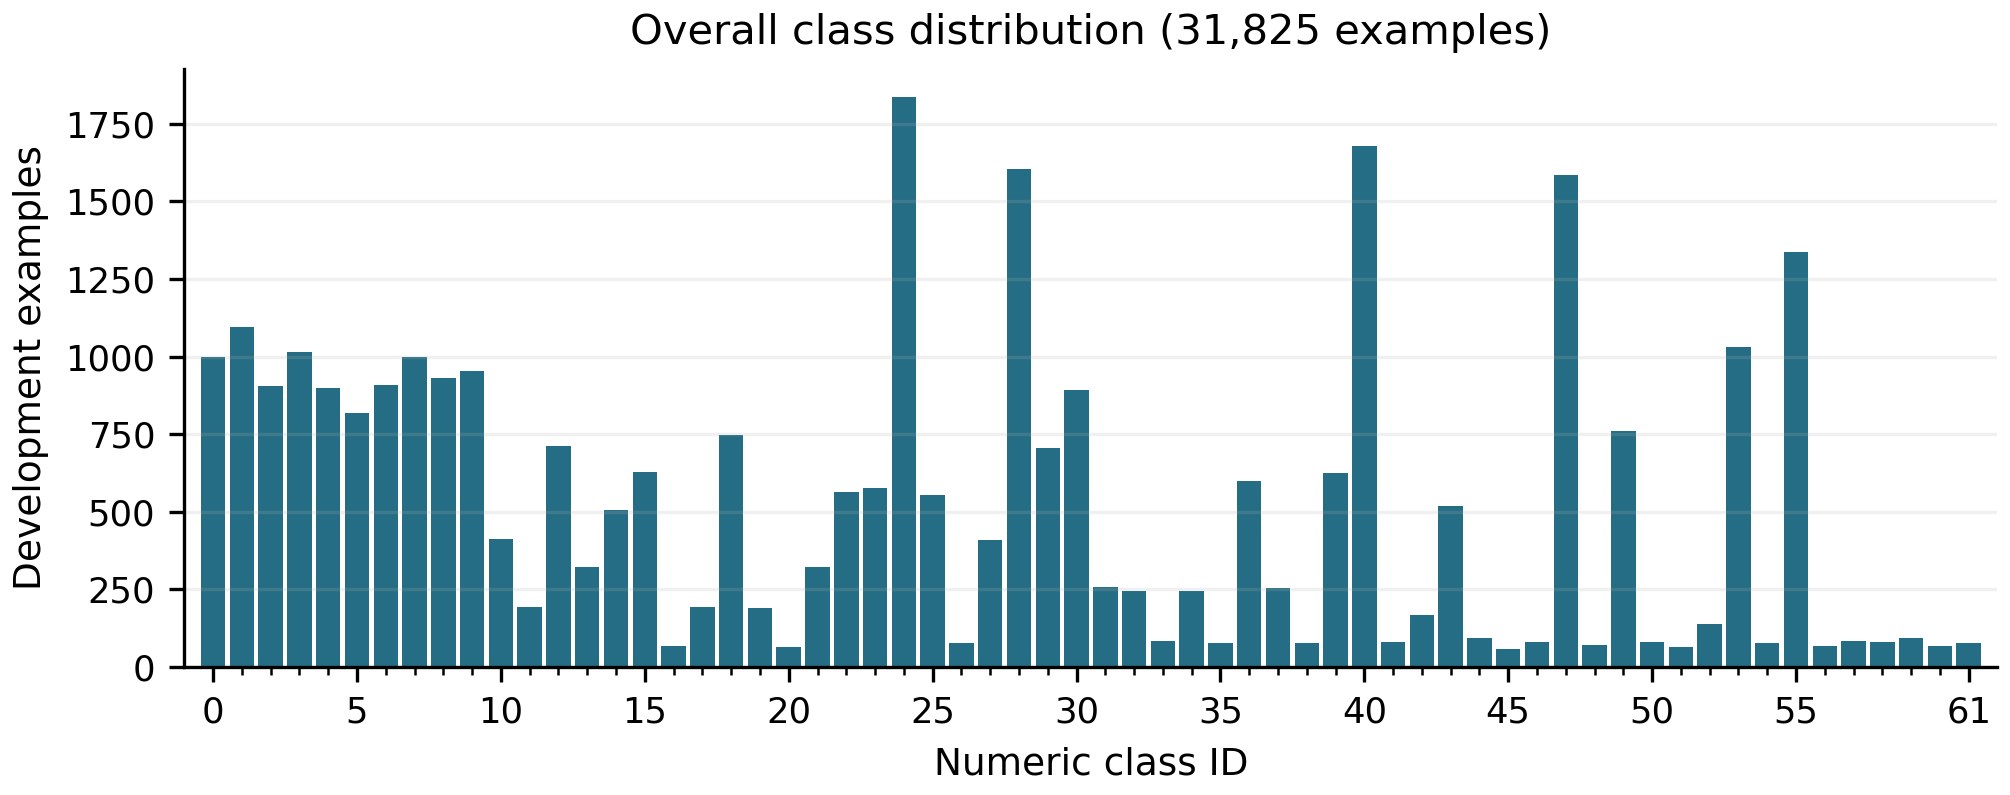
\includegraphics[width=\linewidth]{figures/part1_1/overall_class_distribution.png}
\caption{Counts for all 62 numeric labels in the complete 31,825-example development pool. Peaks and rare classes establish global imbalance; no undocumented character mapping is inferred.}\label{fig:overall}
\end{figure}
\begin{table}[htbp]
\centering
\caption{Five clients selected using training-set characteristics. Entropy is $H_k=-\sum_c p_{kc}\log_2p_{kc}$ over locally observed training labels.}\label{tab:five}
\begin{tabular}{rlrrr}
\toprule
ID & Selection reason & Train / validation & Classes & $H_k$ (bits)\\
\midrule
67 & Largest training set & 314 / 79 & 54 & 5.084\\
25 & Smallest training set & 94 / 24 & 38 & 4.802\\
16 & Most observed classes & 300 / 75 & 57 & 5.221\\
36 & Fewest observed classes & 182 / 46 & 37 & 4.964\\
86 & Median profile & 260 / 65 & 51 & 5.115\\
\bottomrule
\end{tabular}
\end{table}
\begin{figure}[htbp]
\centering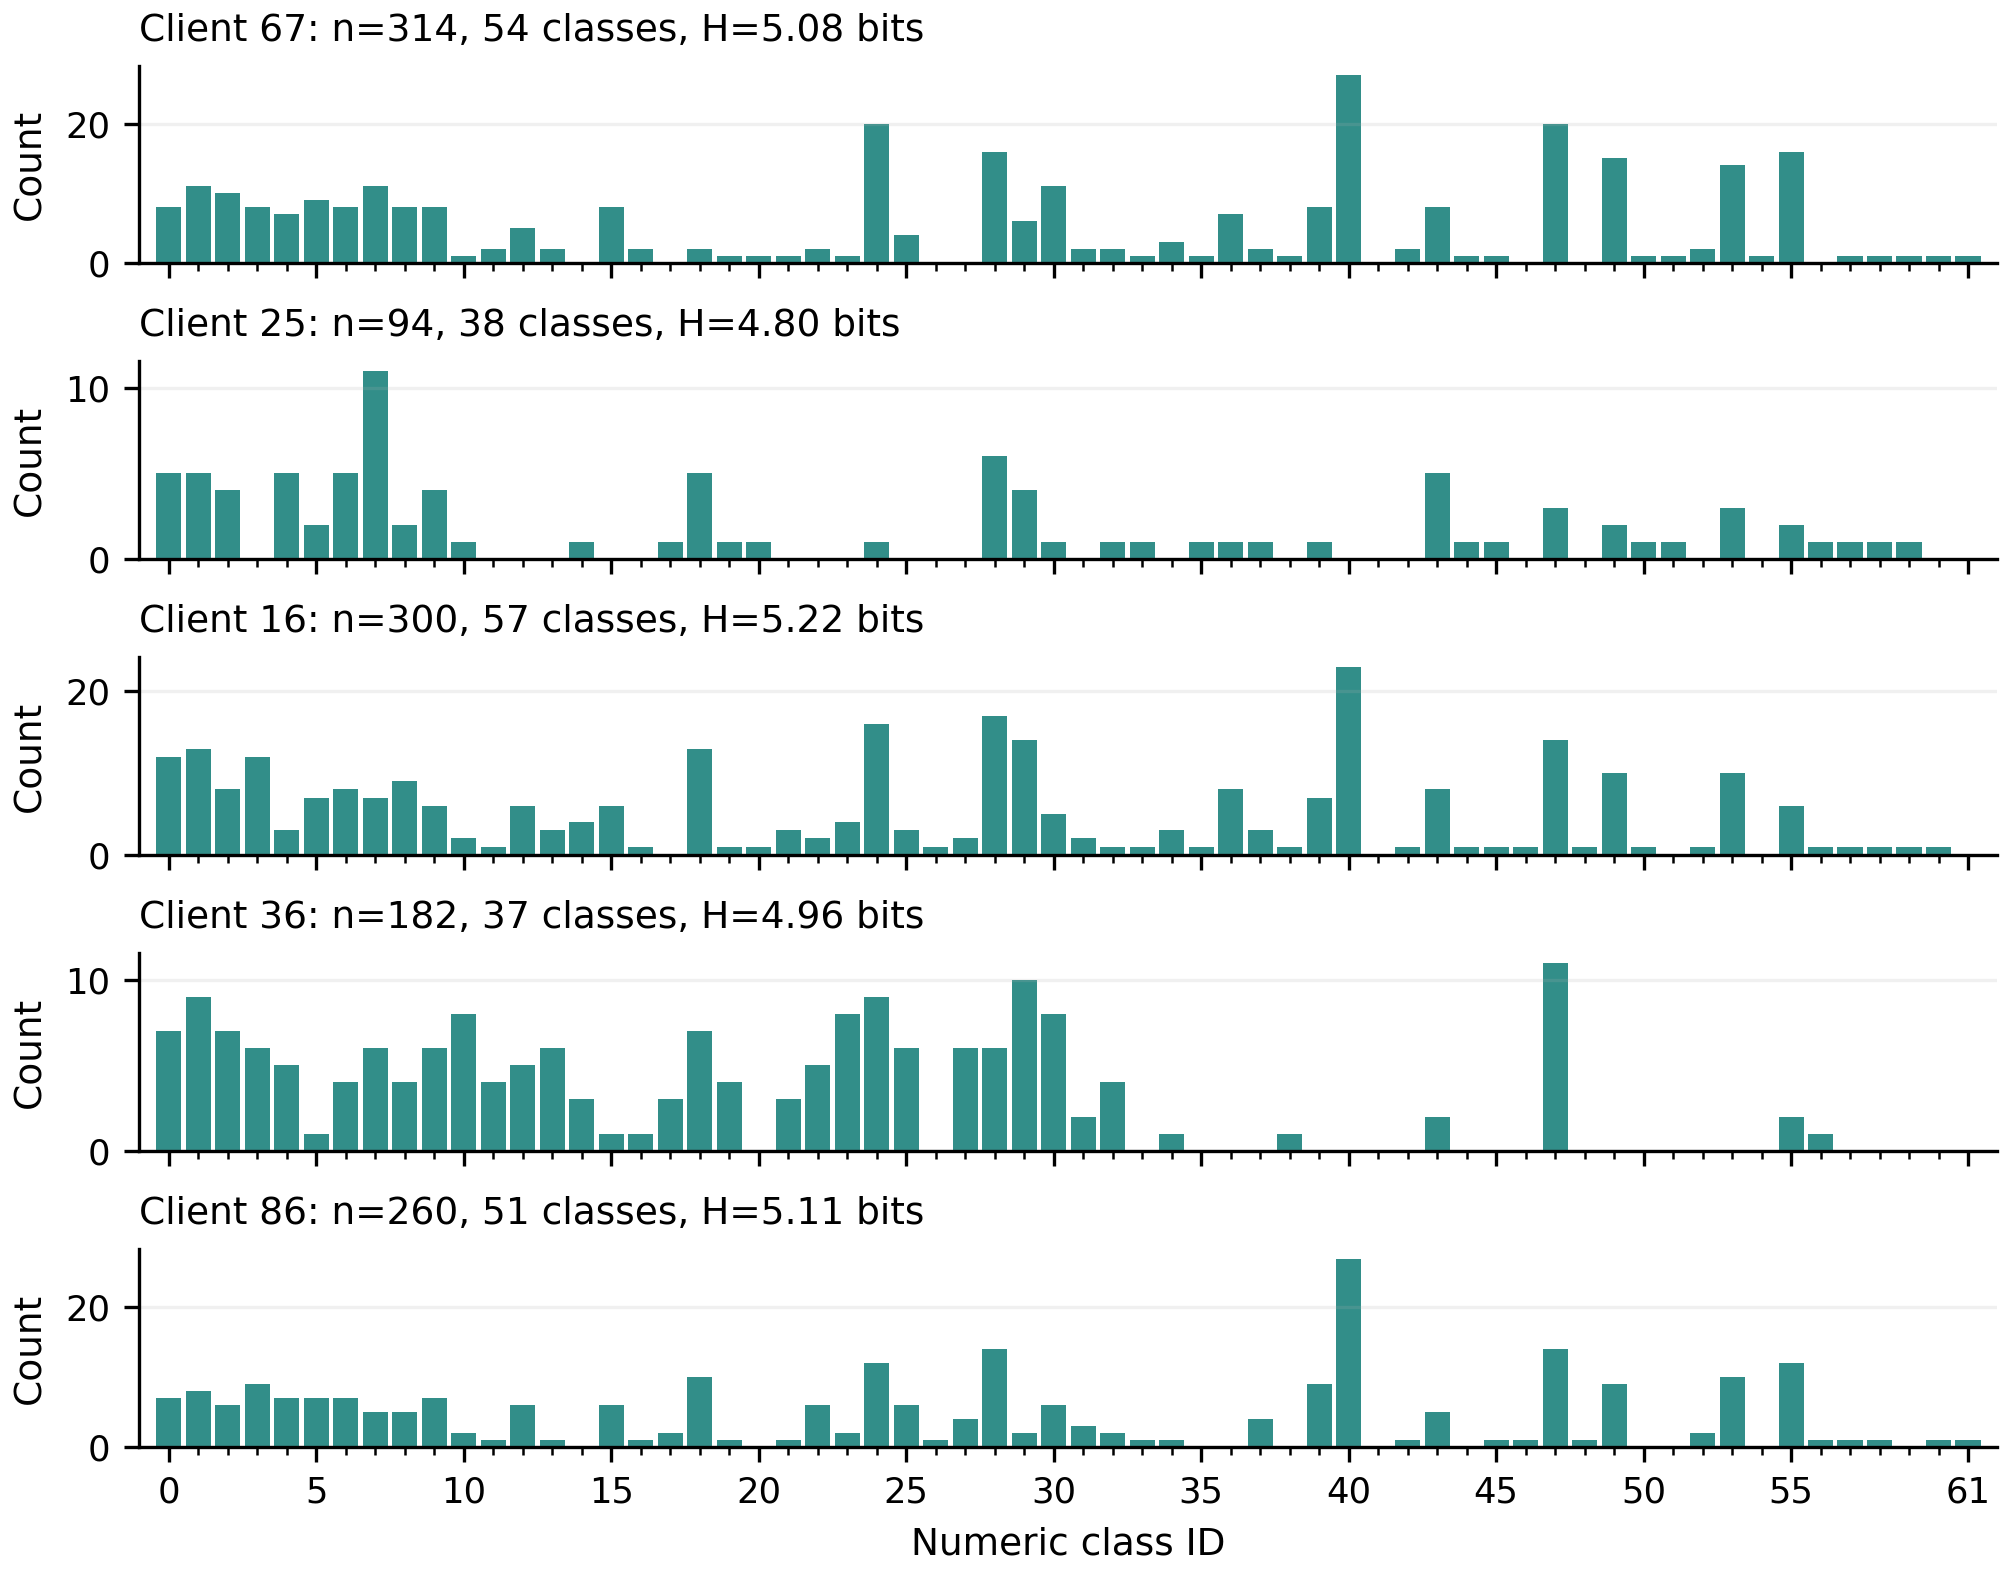
\includegraphics[width=\linewidth]{figures/part1_1/five_client_distributions.png}
\caption{Training-label counts for five systematically chosen clients. The shared numeric-label axis exposes missing classes and differing local proportions. These panels use training subsets, whereas \cref{fig:overall} uses the full development pool.}\label{fig:five}
\end{figure}

Training-label entropy averages 5.111 bits across clients (range 4.682--5.272). The differing proportions, missing labels, and unequal counts characterize empirical heterogeneity; entropy captures label mix rather than handwriting style. The controlled partition experiment below tests how stronger label segregation affects learning.

\subsection{Questions 2--4: baseline convergence and hyperparameter comparison}
The baseline uses $C=0.10$, $E=1$, learning rate 0.3, batch size 32, seed 2026, and 80 rounds. A preceding six-run, 12-round pilot compared learning rates 0.01, 0.1, and 0.3 at $E=1,3$ with $C=0.10$. The mean final validation accuracies over the two epoch settings were 6.86\%, 28.33\%, and 46.69\%, respectively. The largest mean selected the shared rate 0.3 before the main grid; test data were not used.

At the baseline, training/validation accuracy rises from 3.19\%/3.03\% to 67.02\%/65.29\%. Training cross-entropy falls from 4.126150 to 1.246401 and validation cross-entropy from 4.126700 to 1.328689 (\cref{fig:baseline}).
\begin{figure}[htbp]
\centering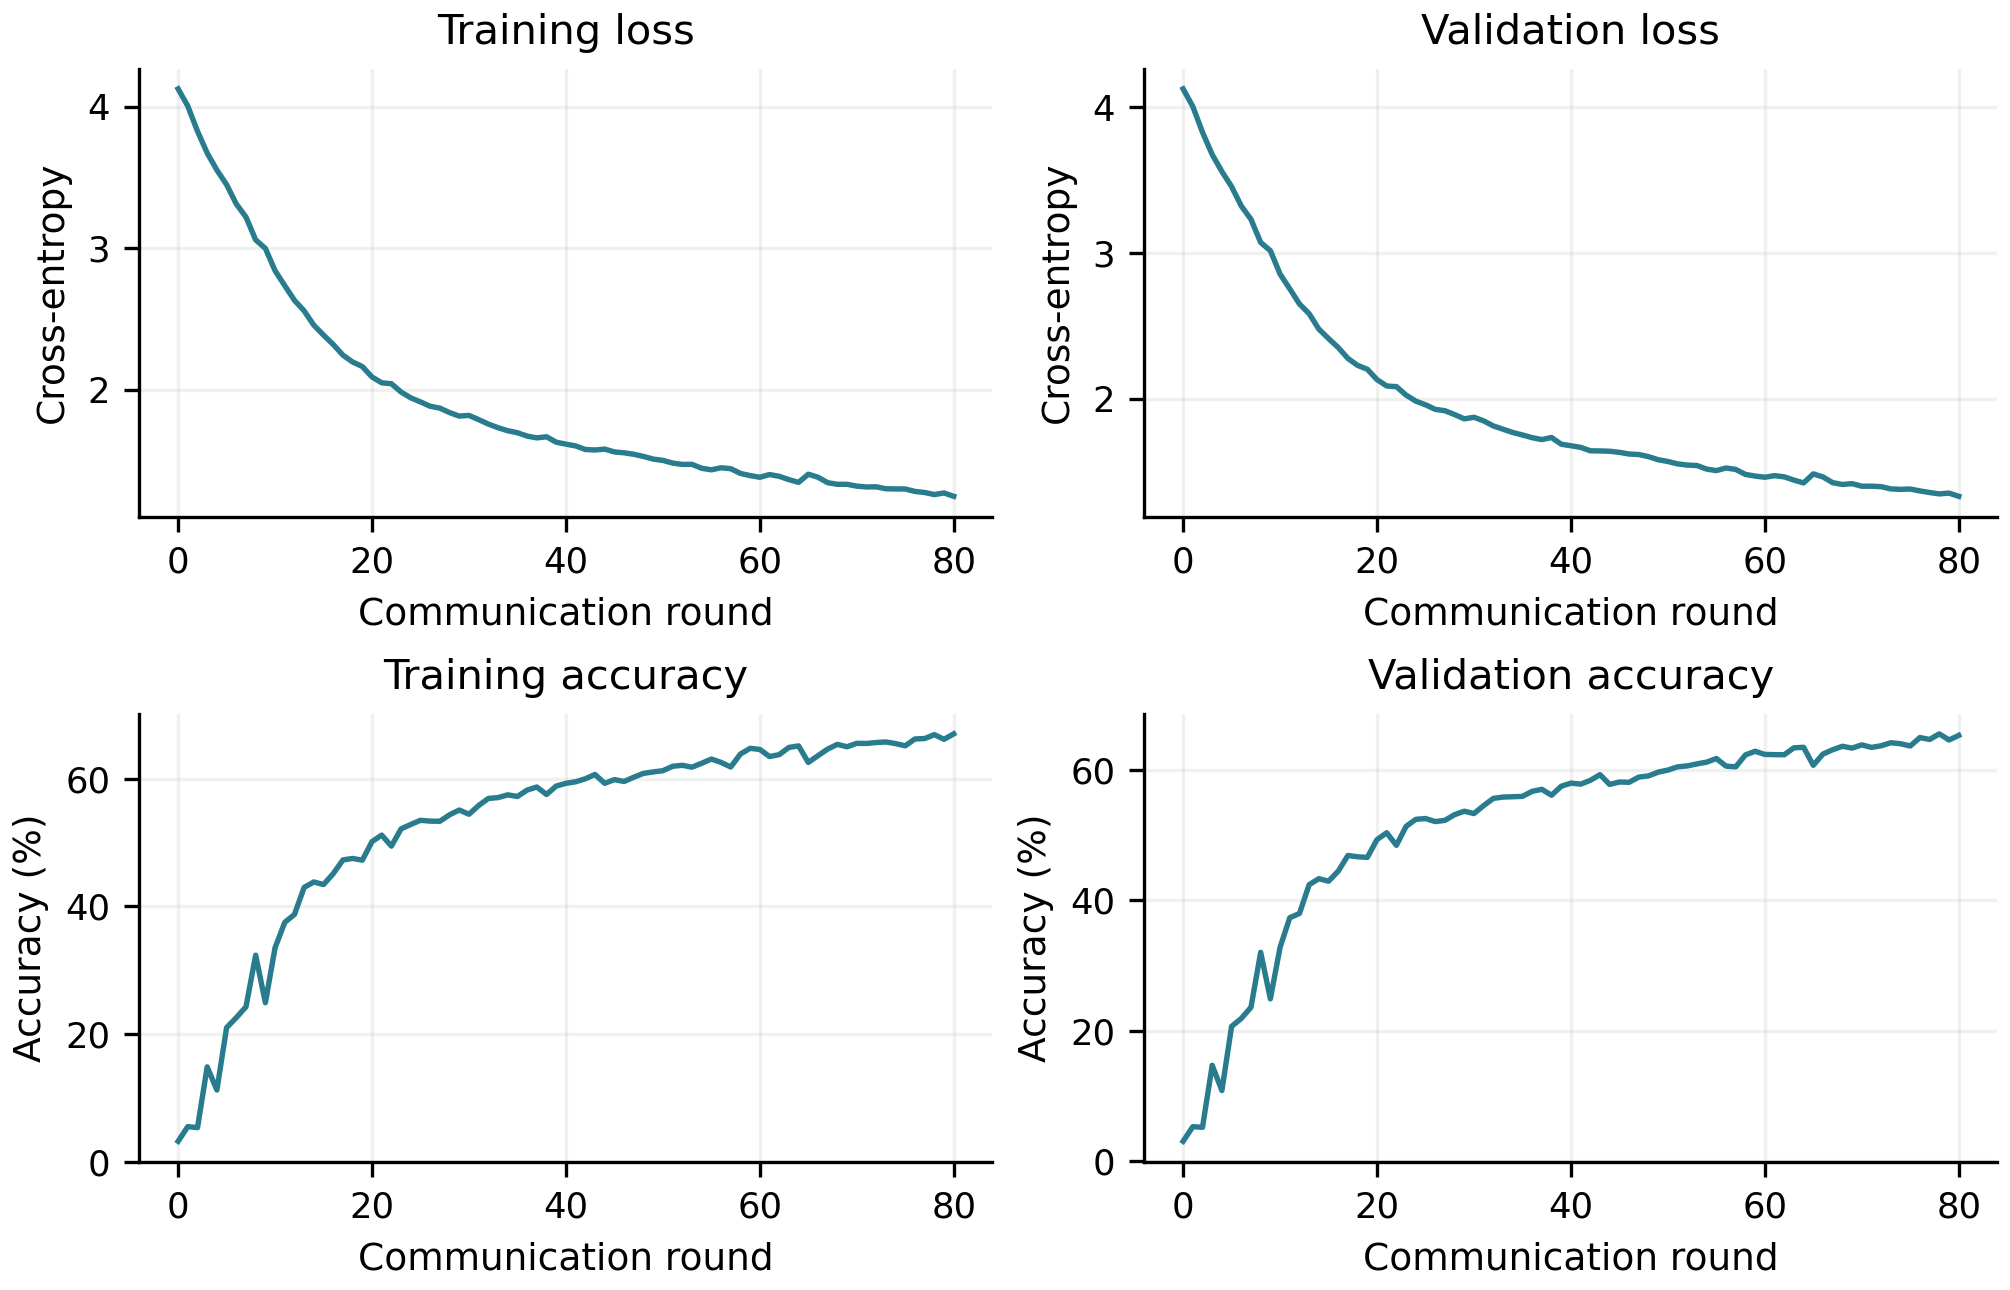
\includegraphics[width=\linewidth]{figures/part1_1/baseline_convergence.png}
\caption{Required full-pool training and validation loss/accuracy curves for sequential FedAvg, $C=0.10$, $E=1$, seed 2026. Round zero is the initialized model. Each later point evaluates the updated global model, not an average of selected clients' local models.}\label{fig:baseline}
\end{figure}

\begin{table}[htbp]
\centering
\caption{Main 80-round comparison, seed 2026, learning rate 0.3 and batch size 32. Accuracies are percentages. Best validation and final validation are distinct.}\label{tab:grid}
\begin{tabular}{rrrrrrr}
\toprule
$C$ & $E$ & Final train & Final val. & Best val. (round) & Client-epochs & Exposures\\
\midrule
0.02 & 1 & 60.83 & 59.03 & 61.28 (78) & 160 & 40,949\\
0.02 & 3 & 69.99 & 67.64 & 69.39 (77) & 480 & 122,847\\
0.05 & 1 & 66.40 & 64.66 & 64.66 (80) & 400 & 102,161\\
0.05 & 3 & 74.85 & 72.59 & 72.98 (78) & 1,200 & 306,483\\
0.10 & 1 & 67.02 & 65.29 & 65.52 (78) & 800 & 203,782\\
0.10 & 3 & 75.32 & 73.00 & 73.00 (80) & 2,400 & 611,346\\
\bottomrule
\end{tabular}
\end{table}
\begin{figure}[htbp]
\centering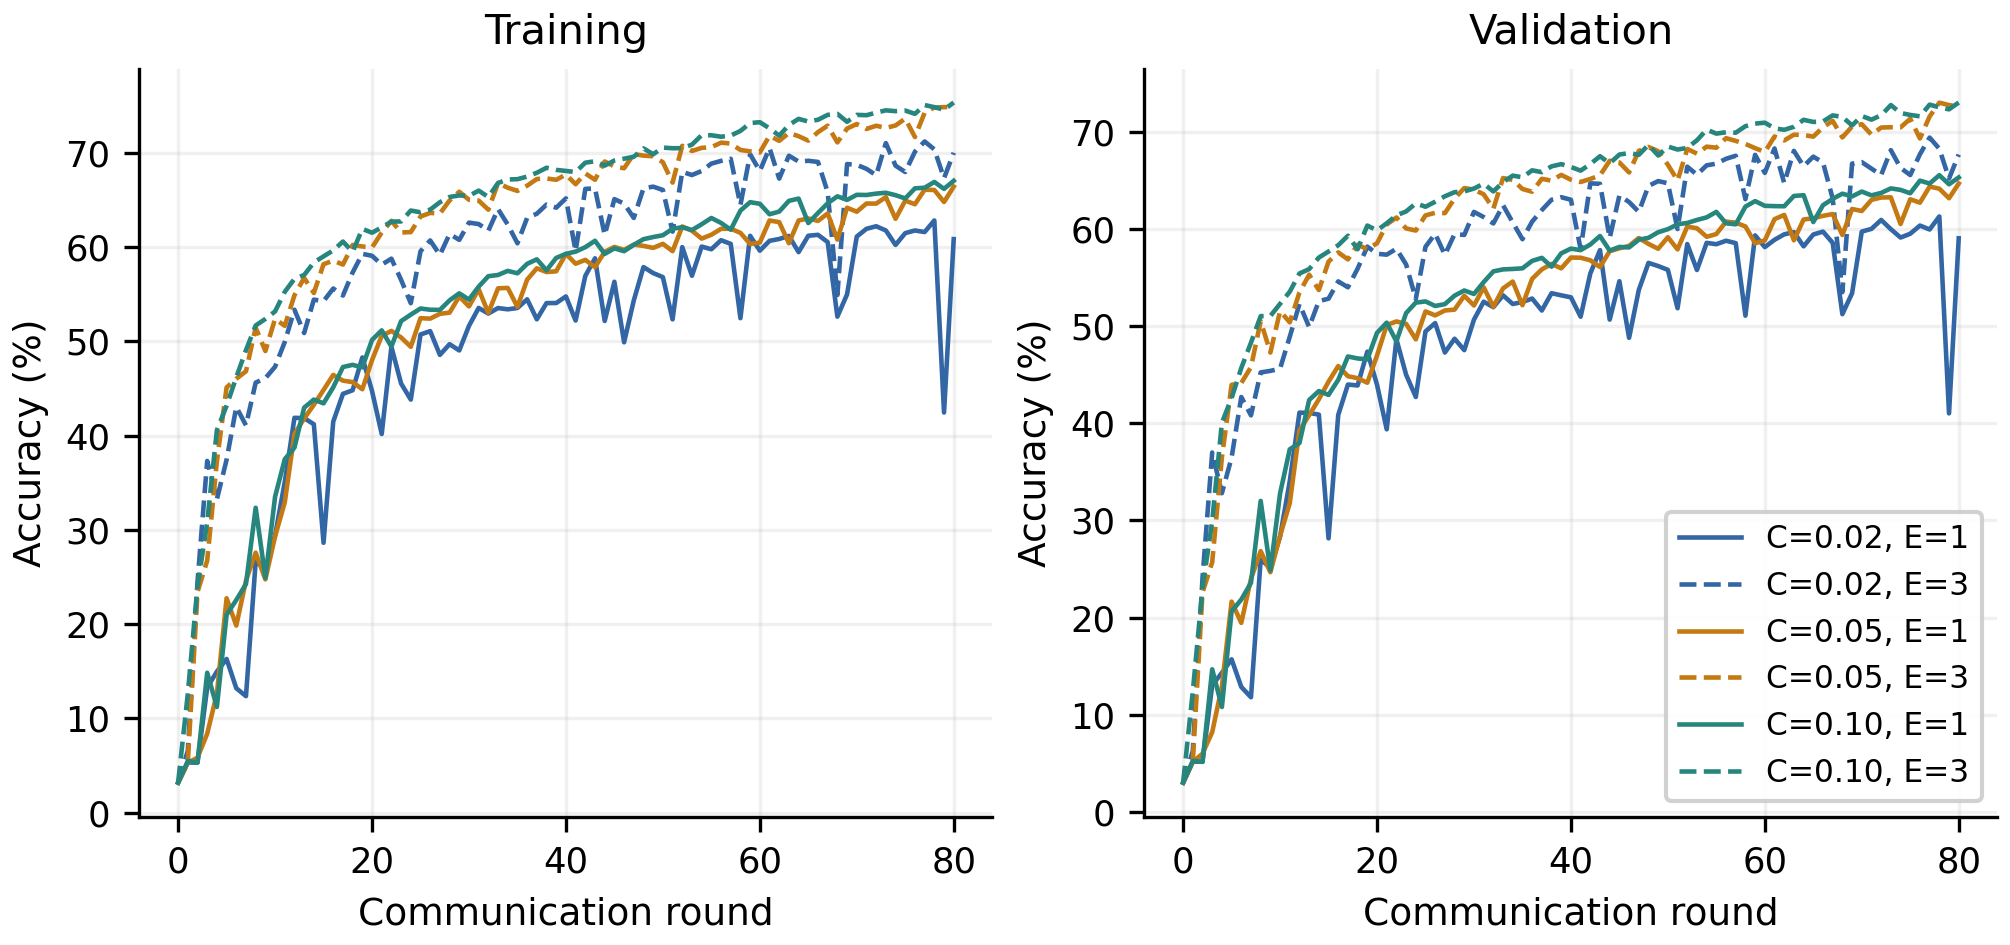
\includegraphics[width=\linewidth]{figures/part1_1/hyperparameter_accuracy.png}
\caption{Training and validation accuracy for the six $(C,E)$ settings. Colors encode client fraction and line style encodes local epochs. The shared round budget is a communication-round comparison, not a matched-computation experiment.}\label{fig:grid}
\end{figure}

Increasing $E$ from 1 to 3 improves final validation accuracy by 8.62, 7.93, and 7.71 percentage points at $C=0.02,0.05,0.10$. These paired-schedule comparisons also triple sample exposures. Larger $C$ generally improves final accuracy and stability while increasing per-round computation. The 80-round grid spans 160--2,400 client-epochs; \cref{tab:grid} reports actual exposures and \cref{fig:cost} shows the corresponding computation tradeoff.

For $C=0.02,E=1$, the largest one-round validation decline is 20.26 points and the last-ten-round SD is 6.05 points; at $C=0.10,E=3$, these decrease to 1.39 and 0.60 points. These trajectory statistics combine trend and sampling fluctuations, rather than independent-run uncertainty. Larger local budgets help here, but stronger heterogeneity can induce client drift \citep{courseFL}.

\subsection{Question 5: validation selection and held-out evaluation}
The two leading primary-seed configurations were repeated at seeds 2027 and 2028. Mean best validation accuracy was $71.94\%\pm0.99\pp$ for $C=0.05,E=3$ and $72.77\%\pm0.23\pp$ for $C=0.10,E=3$; mean final accuracy was $71.52\%\pm1.14\pp$ and $72.40\%\pm0.57\pp$, respectively (sample SD). Maximizing mean best validation selected $C=0.10,E=3$, after which the highest-validation seed/checkpoint was seed 2026, round 80.

The selected model correctly classifies 2,684/3,621 held-out examples: \textbf{74.12\% test accuracy}, with cross-entropy 0.986716. This is the validation-selected seed-2026 result. At fixed round 80, the selected configuration ($C=0.10$, $E=3$, learning rate 0.3, batch size 32) achieves 74.12\%, 72.88\%, and 73.13\% at seeds 2026--2028: a mean of $73.38\%\pm0.66\pp$ (sample SD). These evaluations use the same 3,621 test examples and are supported by Part 2's exactly matched zero-noise trajectories (\cref{sec:p2validation,tab:allnoise}); they describe seed variability rather than independent test datasets.

The primary-seed best-validation advantage over $C=0.05,E=3$ is only $100/6407=0.0156$ points, or one example, so that contrast alone is not evidence of significant superiority. Test evaluation followed the frozen validation selection.

\subsection{Scientific Validation and Edge Cases}\label{sec:p11validation}
\subsubsection{Mathematical correctness: unequal-count aggregation and the SGD identity}
To verify aggregation independently of model accuracy, we compared the implemented update with a manually computed mean of three float32 vectors weighted by counts $[1,3,6]$. The expected vector is $[-0.5,2.8,5.4]$. Maximum error is $2.3841858\times10^{-7}$, below the $10^{-6}$ tolerance, confirming the unequal-count arithmetic.

A second test connects the implementation to a known optimization identity. With all clients participating, one full-batch local SGD step gives
\begin{align}
w_{t+1}^{(k)}&=w_t-\eta\nabla F_k(w_t),\nonumber\\
\sum_k\frac{n_k}{N}w_{t+1}^{(k)}
&=w_t-\eta\sum_k\frac{n_k}{N}\nabla F_k(w_t)
=w_t-\eta\nabla F(w_t),\label{eq:sgdidentity}
\end{align}
Here $F_k$ is a local mean loss and $F$ the pooled mean. With 17 synthetic examples split 2/5/10, the actual 62-output MLP, learning rate 0.03, and one full local batch per client, FedAvg differs from centralized SGD by at most $7.4505806\times10^{-9}$ (tolerance $3\times10^{-7}$). This tests loss normalization, optimization, and aggregation together. The identity applies to this one-step special case; multiple local steps evaluate gradients at different client weights.

\subsubsection{Stochastic correctness: participation and repeatability}
Sampling was checked with 10,000 draws per fraction, verifying subset size, uniqueness, and exact replay of a seeded stream. Under independent rounds, a client's marginal participation count has mean $TC$ and SD $\sqrt{TC(1-C)}$.
\begin{table}[htbp]
\centering
\caption{Sampling diagnostic over 10,000 rounds per fraction. Every subset has the required unique-client count and the same-seed streams match exactly.}\label{tab:sampling}
\begin{tabular}{rrrrr}
\toprule
$C$ & Expected count & Binomial SD & Observed min--max & Maximum $|z|$\\
\midrule
0.02 & 200 & 14.000 & 166--230 & 2.429\\
0.05 & 500 & 21.794 & 432--574 & 3.395\\
0.10 & 1,000 & 30.000 & 924--1,069 & 2.533\\
\bottomrule
\end{tabular}
\end{table}
All participation deviations lie below the five-SD threshold (\cref{tab:sampling}), consistent with the intended marginal sampling probabilities. Exact replay and across-seed learning stability address different questions; \cref{fig:seeds} shows the latter for the two leading settings.

\subsubsection{Positive and negative learning controls}
The positive control tests whether SGD learns a known spatial signal and responds to learning rate. Twenty synthetic clients provide 960 training and 320 validation examples for a balanced binary task, using the unchanged 62-output model. With matched initialization and selections over 25 rounds, learning rate 0.1 reaches 100\% validation accuracy and reduces training loss from 4.051352 to 0.00257871; rate 0.0001 reaches only 1.25\%. The result exceeds the criteria of $>90\%$ accuracy, halving the loss, and a $>20$-point advantage.

The negative control permutes training labels within each client while preserving counts, label frequencies, validation data, initialization, selections, and optimizer settings. After 40 rounds at $C=0.10,E=3$, correct labels yield 66.36\% validation accuracy versus 7.65\% with randomized labels, a 58.72-point gap against a 15-point criterion. Learning thus depends strongly on image--label correspondence. The residual accuracy is compatible with imbalance and preserved local label frequencies; $1/62$ is not an appropriate universal reference for this control.

\subsubsection{Controlled heterogeneity intervention}
To isolate the effect of partition structure, we reassigned the 25,418 training examples to the original client-size vector by either random permutation or label sorting. Validation remained unchanged. Both 40-round runs used the same schedule, $C=0.10,E=3$, and 306,447 example exposures, removing size and computation differences from the comparison.

Label segregation reduces mean entropy from 5.1836 to 0.3780 bits and final validation accuracy from 69.88\% to 27.81\%, a 42.06-point gap (\cref{fig:controls}). This controlled response is consistent with stronger client drift under multi-step SGD. Only this intervention reallocates data; all main experiments retain the original writers.

\begin{figure}[htbp]
\centering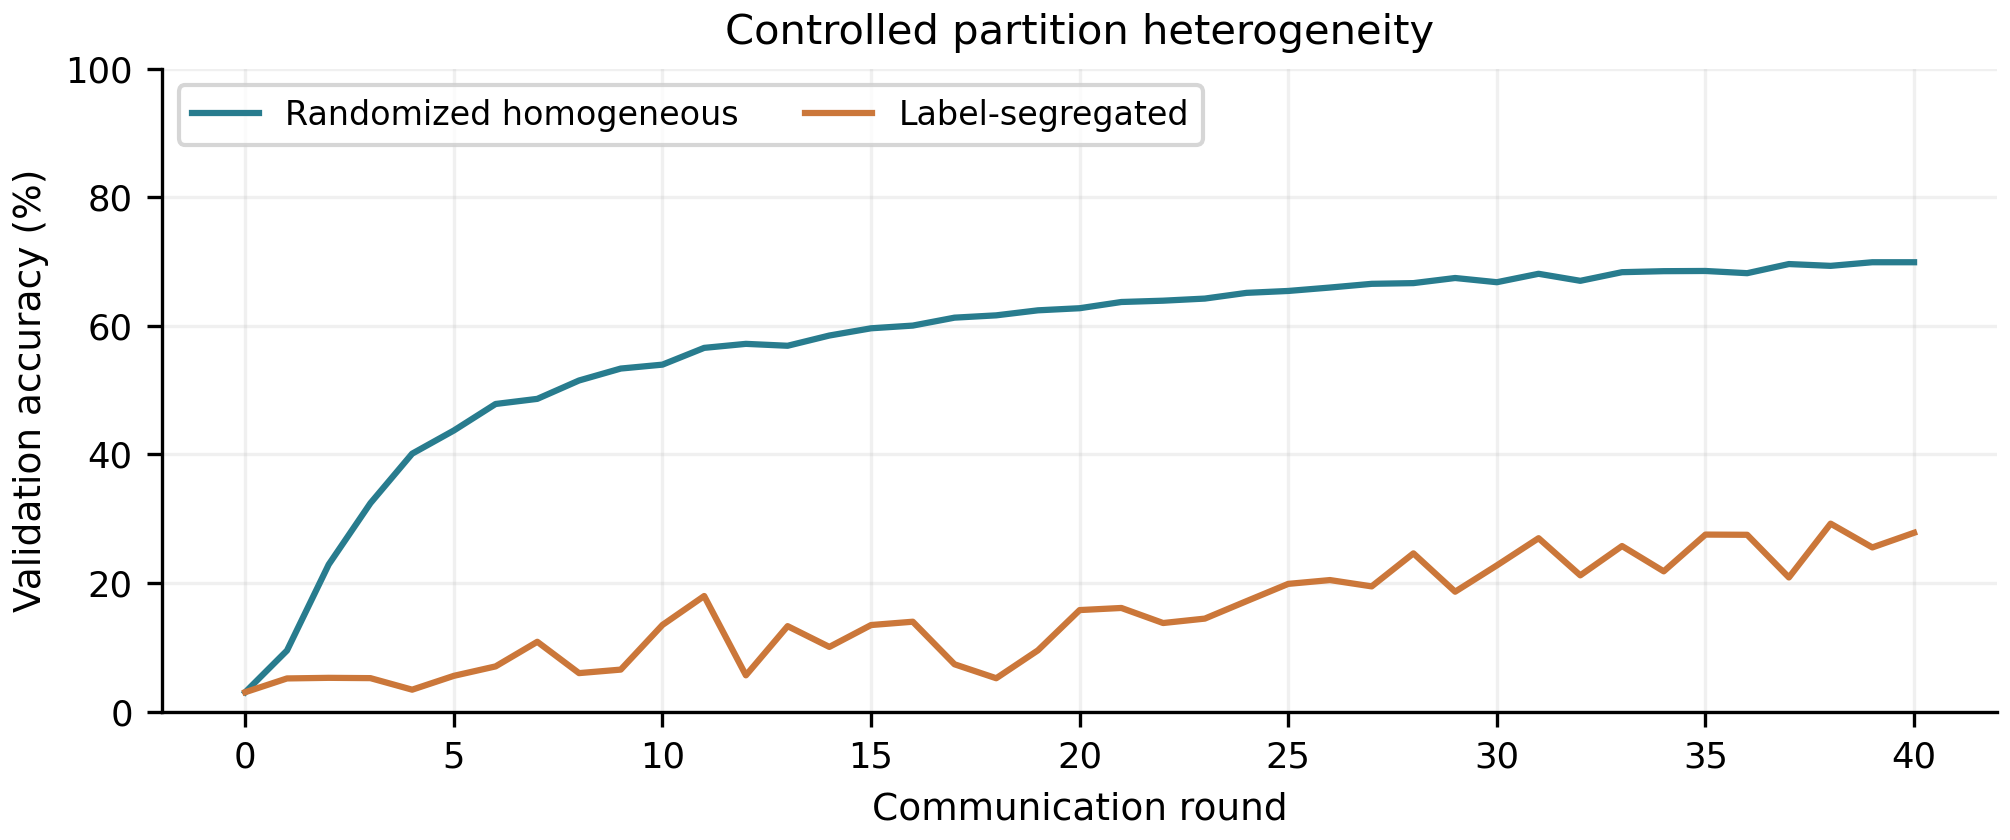
\includegraphics[width=\linewidth]{figures/part1_1/scientific_controls.png}
\caption{Validation accuracy under randomized and label-segregated training partitions. Both preserve client sizes, 306,447 sample exposures, and clean validation data over 40 rounds; $C=0.10$, $E=3$.}\label{fig:controls}
\end{figure}

\subsubsection{Non-standard visualization: who benefits from participation?}
\Cref{fig:benefit} relates participation to local validation improvement for the $C=0.10,E=1$, seed-2026 baseline. Counts range from 2 to 13 against an expectation of 8. Correlations of improvement with participation, training size, and entropy are $-0.0937$, $0.2895$, and $-0.0680$, respectively.

\begin{figure}[htbp]
\centering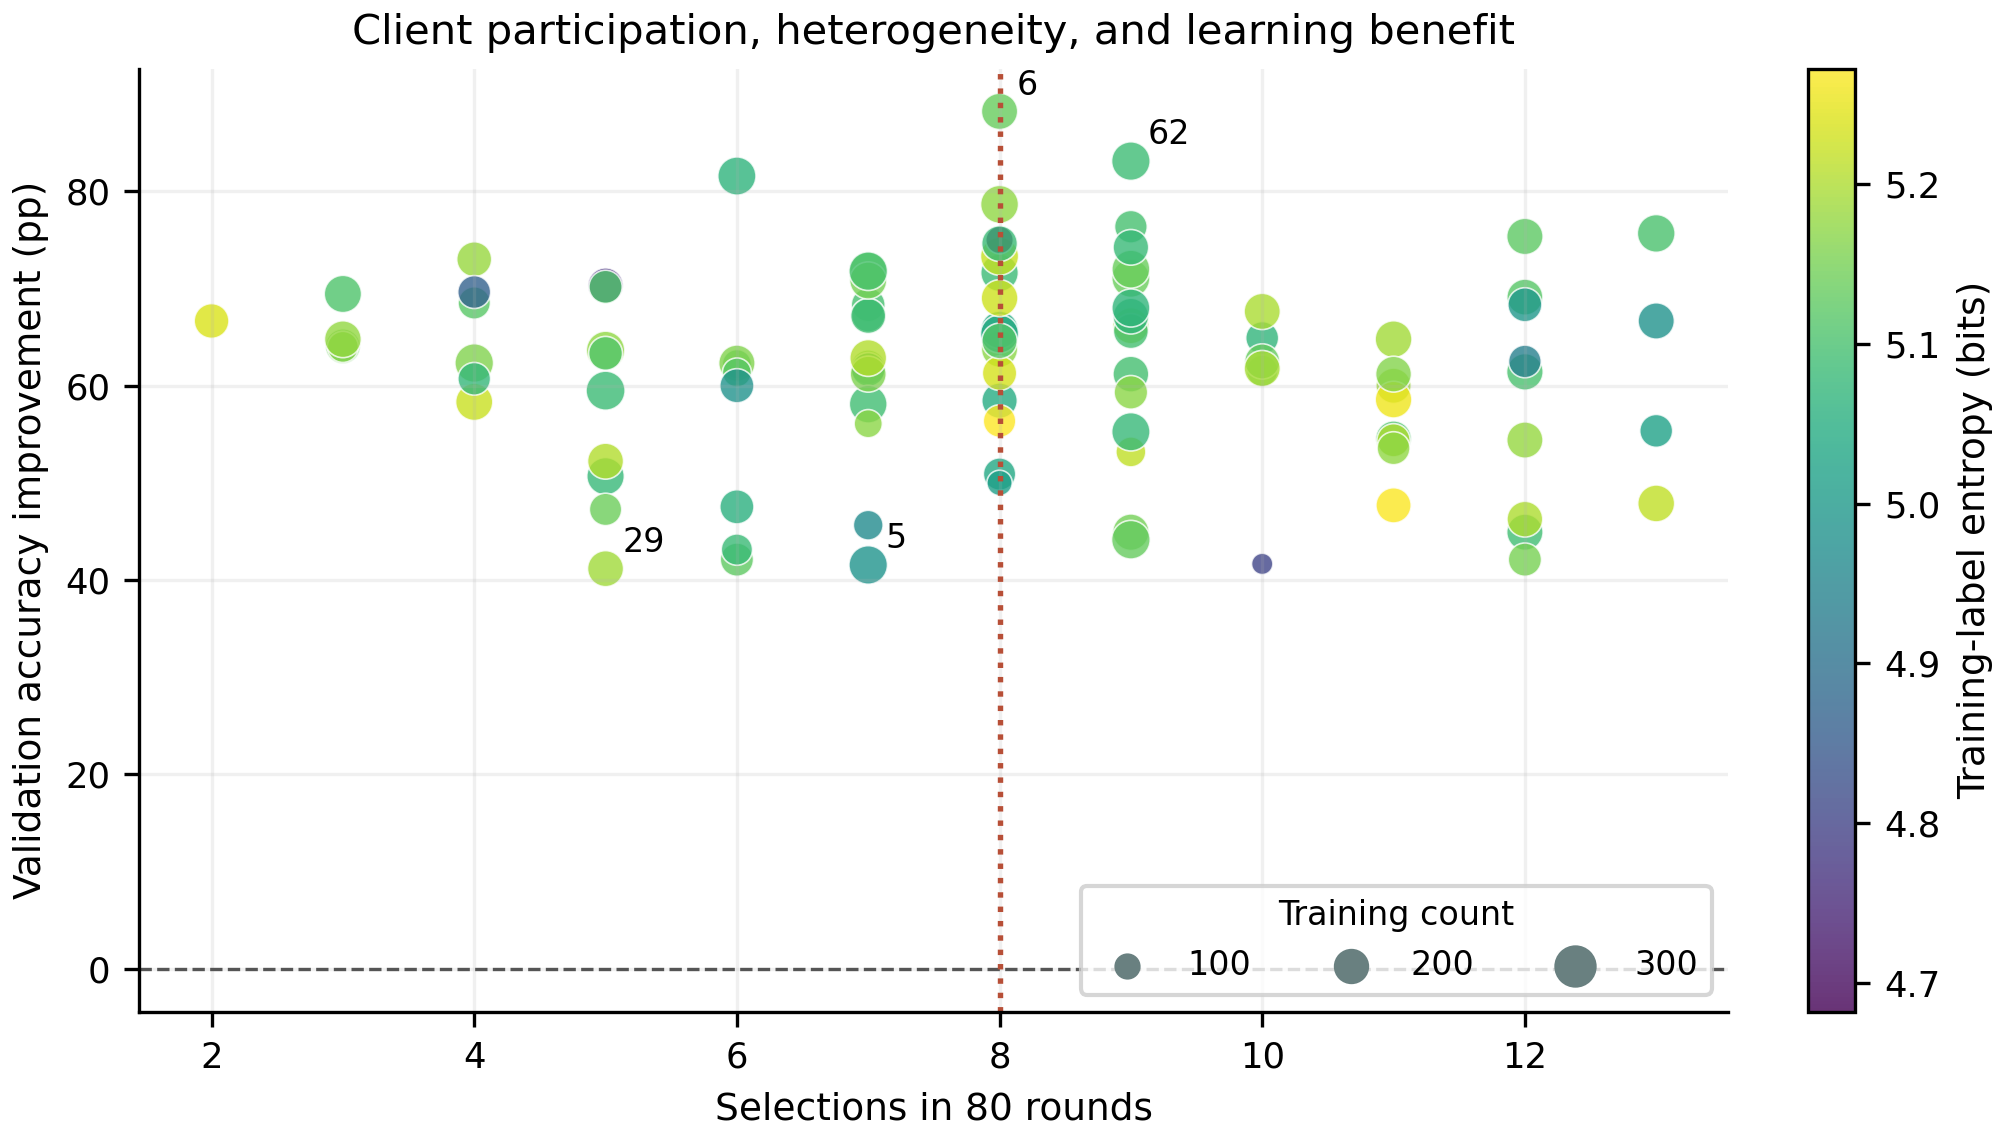
\includegraphics[width=\linewidth]{figures/part1_1/participation_heterogeneity_benefit.png}
\caption{Client participation and validation improvement from round 0 to 80, $C=0.10$, $E=1$, seed 2026. Point area represents training count and color represents label entropy. The reference line marks expected participation $80(0.10)=8$.}\label{fig:benefit}
\end{figure}

Bottom/top training-size quartiles improve by 57.87/65.26 points on average; client 29 improves by 41.18 points and client 6 by 88.24. Benefit is not monotone in participation, because every client receives a global model shaped by others. These exploratory associations describe unequal benefits rather than causal effects of size or participation.

\subsubsection{Robustness, invalid inputs, and restart behavior}
\begin{table}[htbp]
\centering
\caption{Edge-case handling and quantitative checks for Part 1.1. The 13-test suite completed with zero failures or errors.}\label{tab:p11edges}
\begin{tabularx}{\linewidth}{p{0.22\linewidth}YY}
\toprule
Case & Policy / design & Evidence and scope\\
\midrule
Empty and tiny clients & $n=0$ ineligible; $n=1$ training-only; $n\ge2$ has disjoint nonempty subsets. & Coverage/disjointness fixtures include 0, 1, 2, 3, 4, 5, 118, 393. No actual supplied client is empty.\\
Missing classes & Retain all 62 outputs; no fabricated examples. & Singleton class-zero training and empty local validation are checked.\\
Unequal counts & Use positive integer training counts. & A 1:99,999 count fixture averages values 0 and 10 to 9.9999 (five-decimal check).\\
Weighted metrics & Sum counts and losses across clients. & Zero-logit model on sizes 1 and 9 gives accuracy 0.1 and loss $\log62$, not unweighted accuracy 0.5.\\
Invalid updates & Reject NaN/Inf, empty update sets, duplicate IDs, bad counts, incompatible tensors. & Explicit exception assertions; invalid local losses are separately tested.\\
Broadcast / restart & Clone broadcast; create fresh optimizer; commit complete rounds atomically. & Repeated local updates preserve input digest; a three-round stop/resume fixture matches final state digest and selections.\\
Extreme learning rate & Record deterioration or reject non-finite arithmetic. & At $\eta=10^6$, synthetic loss reaches 155,043.09; this run stays finite and does \emph{not} trigger the non-finite guard.\\
\bottomrule
\end{tabularx}
\end{table}

The excessive-rate case in \cref{tab:p11edges} distinguishes finite arithmetic from useful learning: loss remains finite but becomes extremely large. Separate injected-NaN tests verify explicit rejection, while stop/resume tests verify exact recovery at committed round boundaries.




\FloatBarrier
\section{Part 1.2: Parallel Clients with Ray}\label{sec:p12}
\subsection{Actor implementation and required convergence results}
Ray Core Actors are stateful remote objects \citep{rayactors}. Each round creates one Actor for each of four uniformly sampled clients. Actors load their assigned data and run the Part 1.1 local-training routine from the same broadcast. The driver waits for all four updates and aggregates in sampled order, preserving floating-point summation order despite asynchronous completion. A \texttt{finally} block kills the Actors and verifies process exit and CPU-resource return before the next round.

The selected strategy allocates one CPU and zero GPUs per Actor; the alternative benchmark allocates one CPU and 0.25 GPU, sharing one device among four Actors. Both meet the assignment's limits. Actors exist only for selected clients within each round, and all parallelism uses Ray Core directly.

Training uses four clients per round, $E=3$, learning rate 0.3, batch size 32, seed 2026, and 80 rounds (\cref{fig:raycurves}). Final training/validation accuracies are 73.57\%/70.70\%, with losses 0.947290/1.102742. Validation instead selects round 78 at 72.30\%. That checkpoint correctly classifies 2,672/3,621 held-out examples, yielding \textbf{73.79\% test accuracy}.

\begin{figure}[htbp]
\centering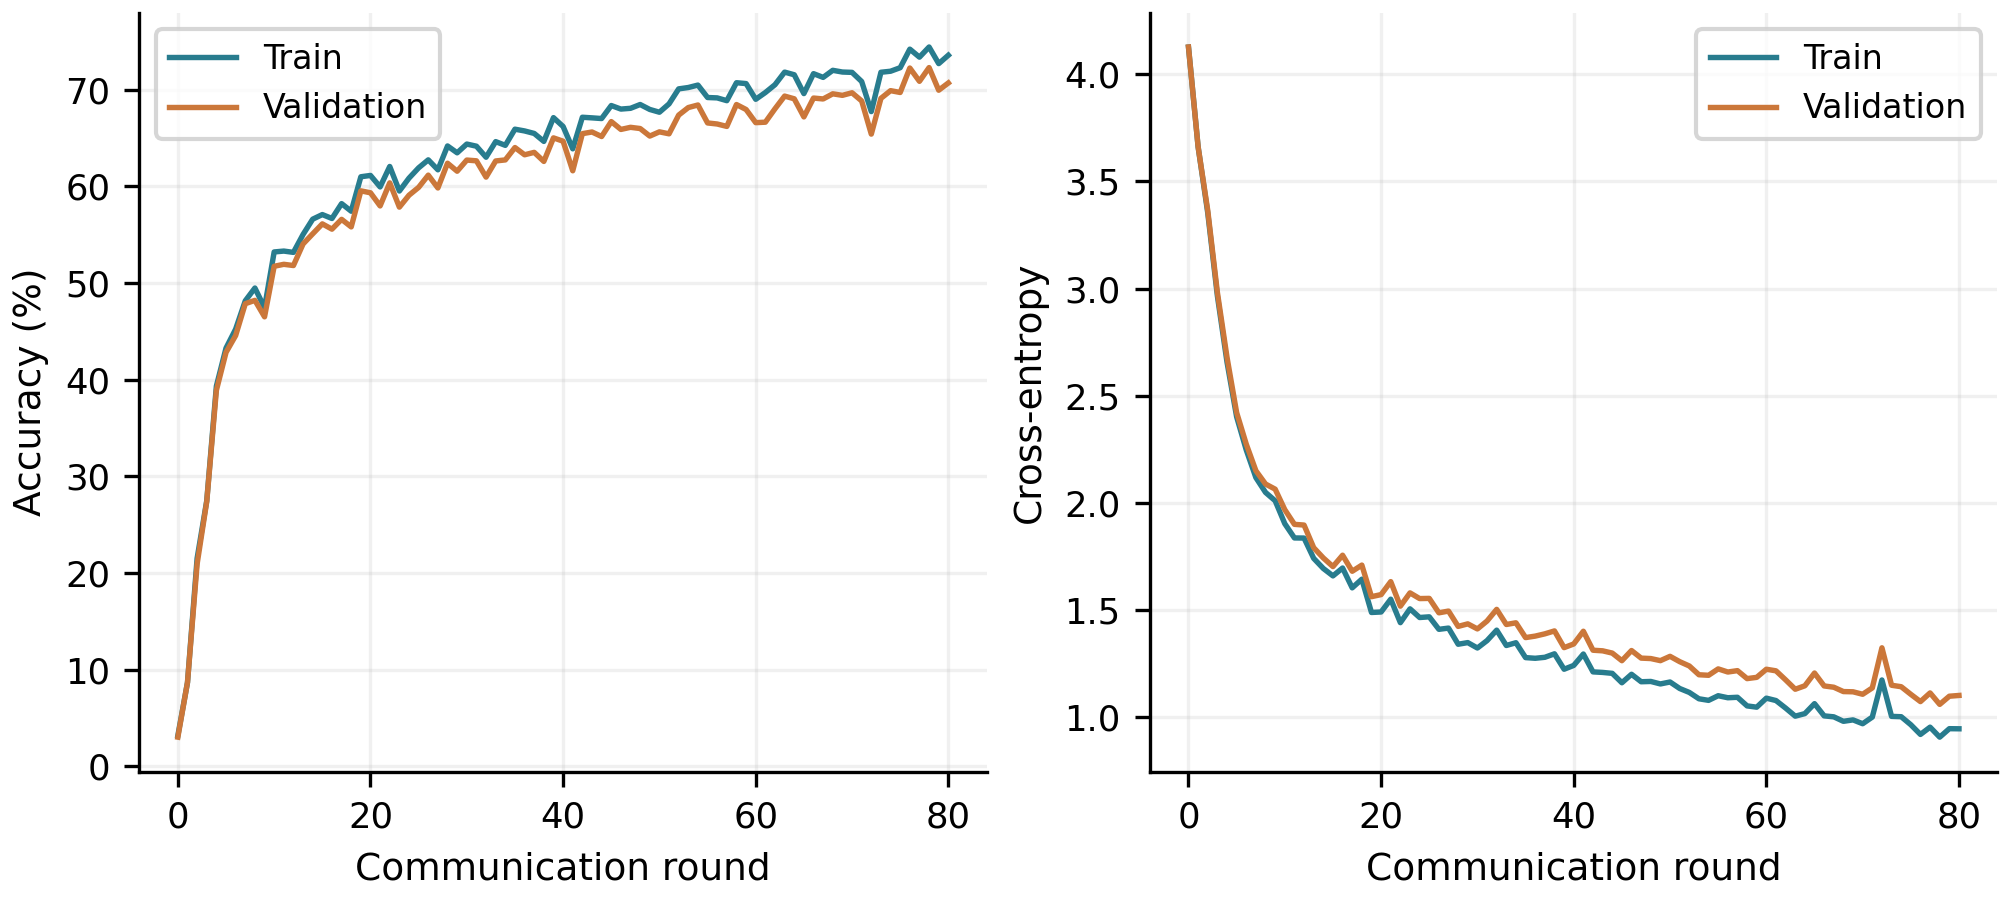
\includegraphics[width=\linewidth]{figures/part1_2/ray_convergence.png}
\caption{Ray training and validation accuracy (left) and cross-entropy (right), including round zero. Four CPU Actors participate per round with $E=3$, learning rate 0.3, and seed 2026. Validation selects round 78.}\label{fig:raycurves}
\end{figure}

\subsection{Scientific Validation and Edge Cases}\label{sec:p12validation}
\subsubsection{A. Numerical correctness of parallel FedAvg}
A matched one-round comparison tests whether parallel execution preserves synchronous FedAvg. Clients 25, 67, 16, and 36 have training sizes 94, 314, 300, and 182. Both implementations use identical initial weights and keyed minibatches at $E=3$ and learning rate 0.3, with an independent weighted-average calculation as an arithmetic reference.

On CPU, every local update, the aggregate, and all training/validation metrics match exactly (maximum difference 0.0; parameter tolerance $10^{-6}$). The independent aggregation error is $1.5521\times10^{-8}$. Fractional-GPU Actors differ from CPU by $2.9802\times10^{-8}$ globally and at most $5.9605\times10^{-8}$ locally, within the $10^{-4}$ cross-device tolerance.

The full 80-round CPU comparison also produces identical selections and metrics, with final parameter difference 0.0 (\cref{fig:raymatch}). Ray therefore preserves the tested serial learning trajectory. The independent Part 1.1 identities address shared-code correctness; the GPU comparison covers only one round.

\subsubsection{B. Actual concurrency, process lifecycle, and memory}
Concurrency was measured from distinct process IDs and training start/finish timestamps, rather than inferred from Actor creation. The intervals begin after the common release barrier. Four training calls overlap in all 80 rounds; every round returns four CPUs and leaves no Actor process alive. \Cref{fig:timeline} illustrates round 1.

\begin{figure}[htbp]
\centering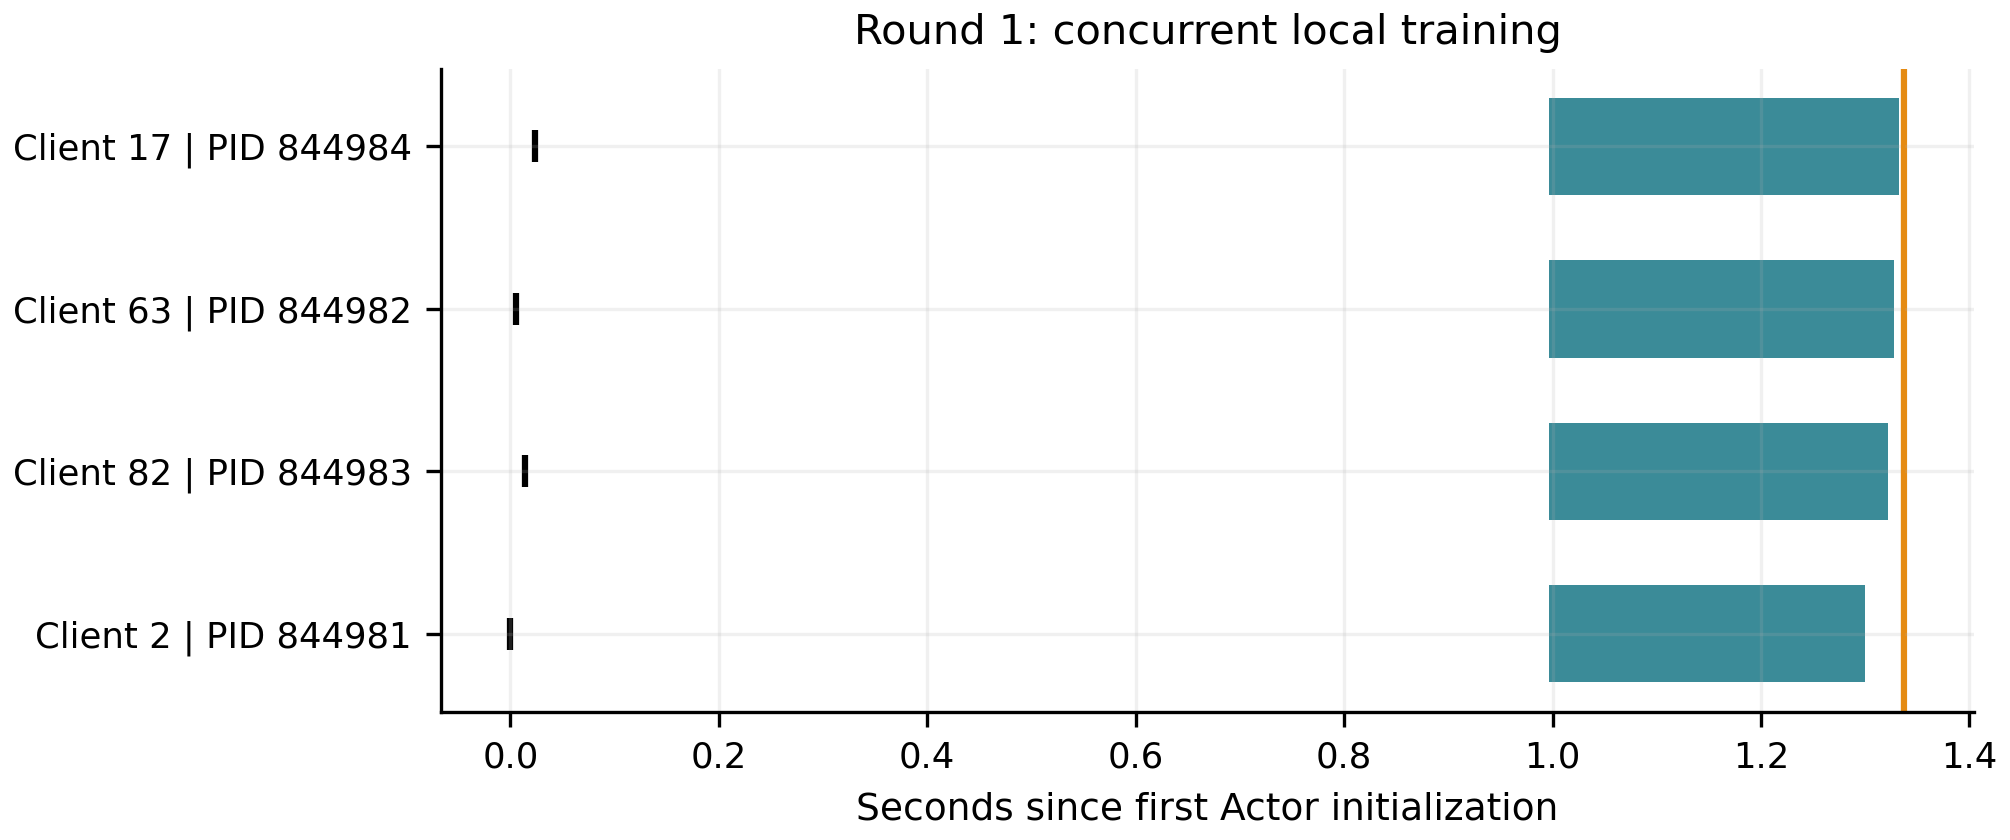
\includegraphics[width=\linewidth]{figures/part1_2/actor_execution_timeline.png}
\caption{Round-1 Actor execution timeline for the CPU run. Black ticks mark initialization, teal intervals local training, and orange aggregation after all updates finish. Four distinct client processes overlap; times are relative to the first Actor initialization.}\label{fig:timeline}
\end{figure}

The mean fastest-to-slowest completion gap is 0.03293 seconds (maximum 0.14037), quantifying one component of synchronous straggler waiting. Driver RSS rises by only 1.43 MiB, from 1,171.49 to 1,172.92 MiB. Together with process exit and resource return, this indicates successful lifecycle cleanup over the run.

\subsubsection{C. Efficiency: concurrent execution is slower here}
Concurrency does not guarantee speedup: savings in local computation must exceed lifecycle and coordination costs. Three repeats of the same four-client round compare one-thread sequential CPU, four one-thread CPU Actors, and four fractional-GPU Actors. Every repeat creates fresh Actors. Among numerically valid strategies, the lower median complete round time selects CPU; \cref{tab:raytiming} reports means and sample SDs.

\begin{table}[htbp]
\centering
\caption{Measured strategy benchmark and full-workload timings. Three-repeat round timers include the Actor lifecycle and release barrier, but exclude global evaluation/checkpointing. Runtime initialization is measured separately and added once.}\label{tab:raytiming}
\begin{tabularx}{\linewidth}{Yrrr}
\toprule
Strategy & Round mean $\pm$ SD (s) & Ray init. (s) & Three rounds + init. (s)\\
\midrule
Sequential CPU & $0.03342\pm0.00173$ & 0 & 0.10027\\
Ray CPU & $3.00794\pm0.41718$ & 5.11084 & 14.13466\\
Ray shared GPU & $4.11489\pm0.69292$ & 3.34036 & 15.68502\\
\midrule
\multicolumn{4}{l}{Full 80-round workload: sequential CPU 11.94713 s; Ray CPU 276.13739 s.}\\
\bottomrule
\end{tabularx}
\end{table}

The full Ray workload takes 272.81936 seconds plus 3.31802 seconds for runtime initialization, totaling 276.13739 seconds, versus 11.94713 seconds sequentially. Both include model initialization, round-zero and later evaluation, and checkpoint/history I/O; Ray also includes cleanup and shutdown. Python launch and prior data preparation are excluded. Thus
\begin{equation}
\text{speedup}=\frac{11.94713}{276.13739}=0.04326,
\qquad\text{slowdown}=23.11.\label{eq:speedup}
\end{equation}
These full-workload times differ from the isolated round benchmark, which excludes global evaluation and checkpoint I/O. Runtime initialization is added once in each comparison.

\begin{figure}[htbp]
\centering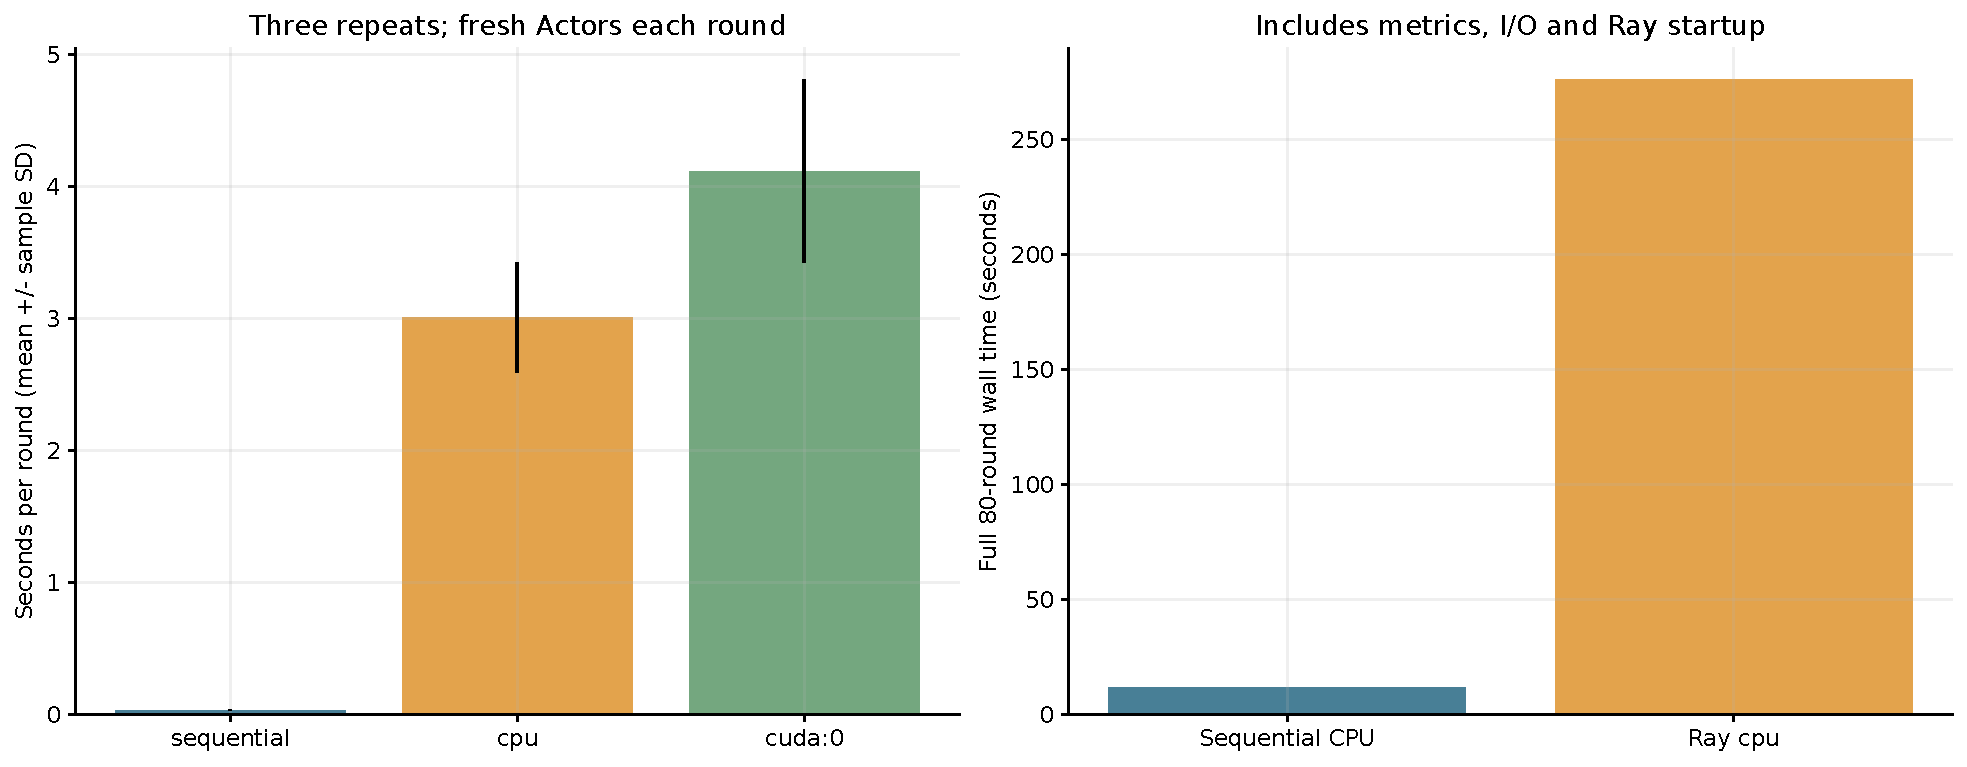
\includegraphics[width=\linewidth]{figures/part1_2/parallel_performance.pdf}
\caption{Complete round time (left; mean and sample SD over three repeats with fresh Actors) and full 80-round workload time (right; including evaluation, I/O, and Ray initialization once).}\label{fig:rayperformance}
\end{figure}

Mean Actor startup is 2.68811 seconds, versus 0.31683 seconds per local training interval; cleanup and aggregation average 0.09368 and 0.00117 seconds. Startup therefore dominates this small 108,478-parameter workload. The 0.15-second common release delay is also included in round time. Imports, model construction, serialization, and scheduling contribute overhead; GPU Actors additionally incur context and transfer costs. The timers do not isolate every component, but clearly explain the measured slowdown (\cref{fig:rayperformance}).

\subsubsection{Failures, unavailable resources, and deterministic recovery}
\begin{table}[htbp]
\centering
\caption{Ray failure injection and edge cases. Allocation failures and unavailable GPUs are controlled injections or logical resource shortages.}\label{tab:rayedges}
\begin{tabularx}{\linewidth}{p{0.24\linewidth}YY}
\toprule
Case & Experiment and expected response & Recorded result\\
\midrule
Actor exception & One of four Actors raises a runtime error; reject the round and clean up. & Explicit Ray task error; four CPUs returned.\\
Allocation failure & Inject \texttt{MemoryError}, without exhausting physical RAM. & Explicit error; four CPUs returned.\\
Non-finite update & Fill one returned parameter with NaN. & Aggregator raises \texttt{FloatingPointError}; no valid aggregate.\\
Unavailable GPU & Request fractional GPUs in a CPU-only runtime with a 0.5 s deadline. & \texttt{GetTimeoutError}; four CPUs returned.\\
Interrupted round & Inject interruption before aggregation/commit, then replay. & Explicit interruption; replay parameter difference 0.0.\\
Tiny / missing classes & Synthetic sizes 1, 2, 7, 13, all class zero; compare serial/Ray. & Maximum parameter difference 0.0.\\
Unequal sizes & Real counts 94, 314, 300, 182; count-weighted reference. & CPU manual aggregation error $1.55\times10^{-8}$.\\
Sampling & 10,000 rounds, four unique clients, same/different seed checks. & Counts 351--439 versus mean 400; maximum $|z|=2.501$.\\
\bottomrule
\end{tabularx}
\end{table}

Failure tests in \cref{tab:rayedges} verify that incomplete rounds never contribute partial averages. Automatic Actor retries are disabled; deterministic replay starts from the last committed checkpoint and leaves the broadcast unchanged. The resource failures are controlled injections or logical shortages, not actual RAM exhaustion or hardware outages.




\section{Part 2: Laplace Input Perturbation}\label{sec:p2}
\subsection{Mechanism and fixed experimental protocol}
For a raw normalized image $X$, the assignment prescribes independent noise at each pixel:
\begin{equation}
 X'=X+\xi,\qquad \xi_{ij}\overset{\mathrm{iid}}{\sim}\operatorname{Laplace}(0,b),
 \qquad p(\xi\mid b)=\frac{1}{2b}\exp\left(-\frac{|\xi|}{b}\right),\quad b>0.\label{eq:laplace}
\end{equation}
Because the network receives $z=1-X$, raw-image addition becomes $z'=1-X'=z-\xi$. At $b=0$, the implementation returns an unchanged clone without random draws.

Each run generates one fixed perturbed copy of each client's training data and reuses it for 80 rounds. Labels remain unchanged and noisy inputs are never clipped to $[0,1]$. Scale is in normalized pixel units. Training, validation, and test evaluation all use clean inputs.

Sequential FedAvg uses $C=0.10$, $E=3$, learning rate 0.3, and batch size 32. Seven scales, $b\in\{0,0.025,0.05,0.10,0.20,0.40,0.80\}$, are evaluated at seeds 2026--2028. Initialization, participation, and minibatches are matched across scales. NumPy PCG64 generates noise on CPU from keys incorporating seed, client ID, and scale; identical values are transferred to CUDA. Because scale enters the key, different scales have separate noise realizations.

The protocol fixes round 80 for all 21 scale-comparison checkpoints and separately evaluates the validation-best $b=0.10$, seed-2026 model for Question 1. Before test scoring, the scale recommendation is fixed by a maximum two-percentage-point decrease in mean final validation accuracy relative to $b=0$.

\subsection{Question 1: the detailed perturbed-data run}
For $b=0.10$, seed 2026, validation selects round 80. Clean training/validation accuracies are 72.37\%/70.72\% and losses are 0.986190/1.119120. Test accuracy is \textbf{71.64\%} (2,594/3,621), distinct from the 70.97\% three-seed mean at this scale. \Cref{fig:dpaccuracy} shows accuracy against the matched clean run; \cref{fig:dploss} provides supporting cross-entropy curves.

\begin{figure}[htbp]
\centering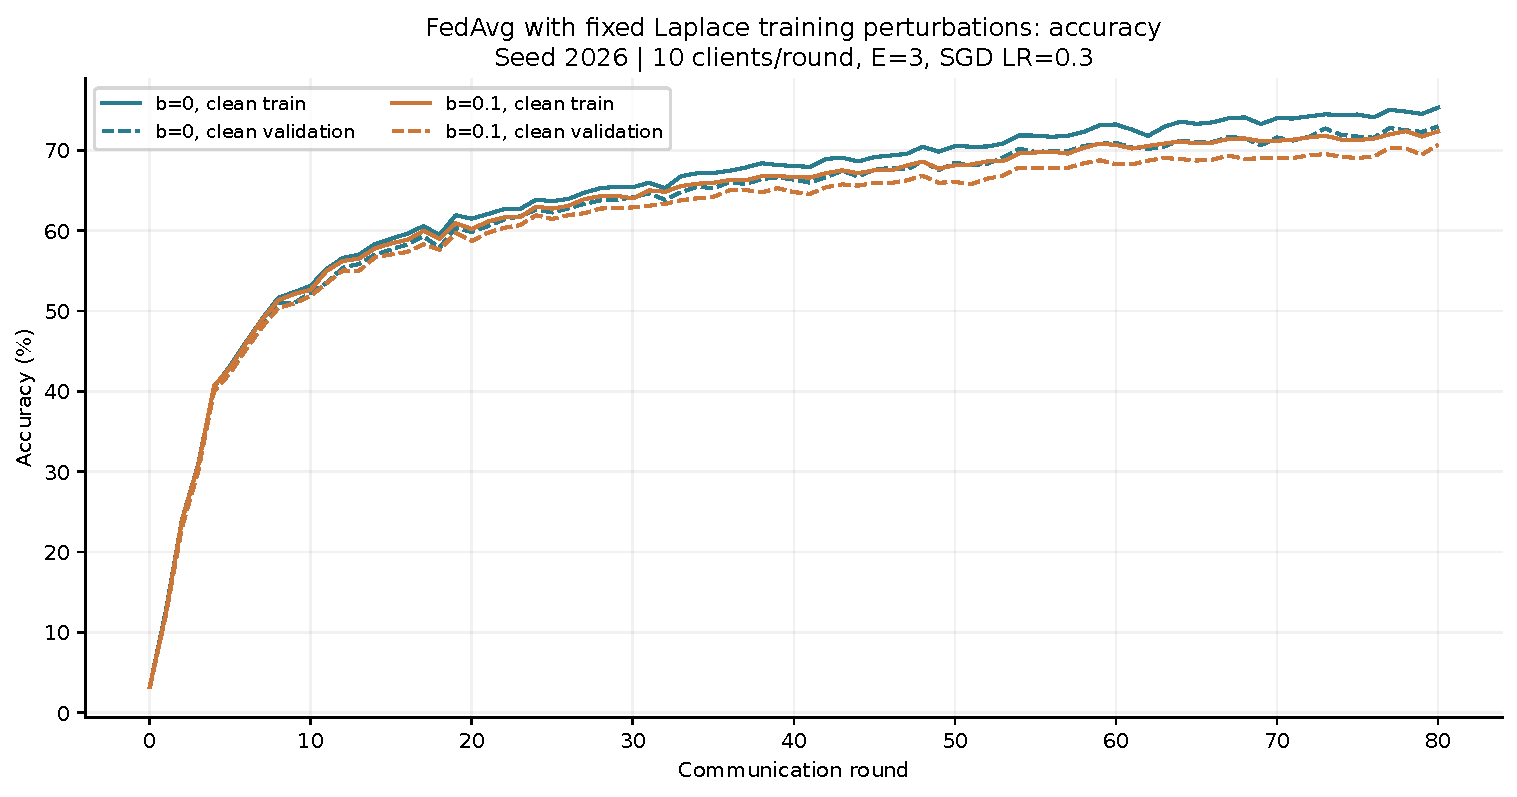
\includegraphics[width=0.9\linewidth]{figures/part2/dp_accuracy_convergence.pdf}
\caption{Part 2 Question 1: clean training and validation accuracy after training on fixed perturbed inputs, $b=0.10$ versus $b=0$, seed 2026. Both use ten clients per round and $E=3$. The noisy run's validation-best checkpoint is round 80.}\label{fig:dpaccuracy}
\end{figure}


\subsection{Questions 2--3: utility across scales and the recommendation}
\begin{table}[htbp]
\centering
\caption{Round-80 clean accuracy across seeds 2026--2028. Training values are means; validation and test show mean accuracy (\%) $\pm$ one sample SD (percentage points).}\label{tab:noisegrid}
\begin{tabular}{rrrr}
\toprule
$b$ & Training (\%) & Validation (\%) & Held-out test (\%)\\
\midrule
0 & 74.97 & $72.40\pm0.57$ & $73.38\pm0.66$\\
0.025 & 74.83 & $72.13\pm0.60$ & $73.16\pm0.65$\\
0.05 & 74.15 & $71.80\pm0.73$ & $72.66\pm0.55$\\
0.10 & 72.16 & $70.05\pm0.58$ & $70.97\pm0.57$\\
0.20 & 66.55 & $64.76\pm0.83$ & $66.06\pm0.90$\\
0.40 & 58.91 & $57.98\pm0.50$ & $58.79\pm0.54$\\
0.80 & 36.77 & $35.57\pm1.76$ & $37.15\pm1.92$\\
\bottomrule
\end{tabular}
\end{table}
\begin{figure}[htbp]
\centering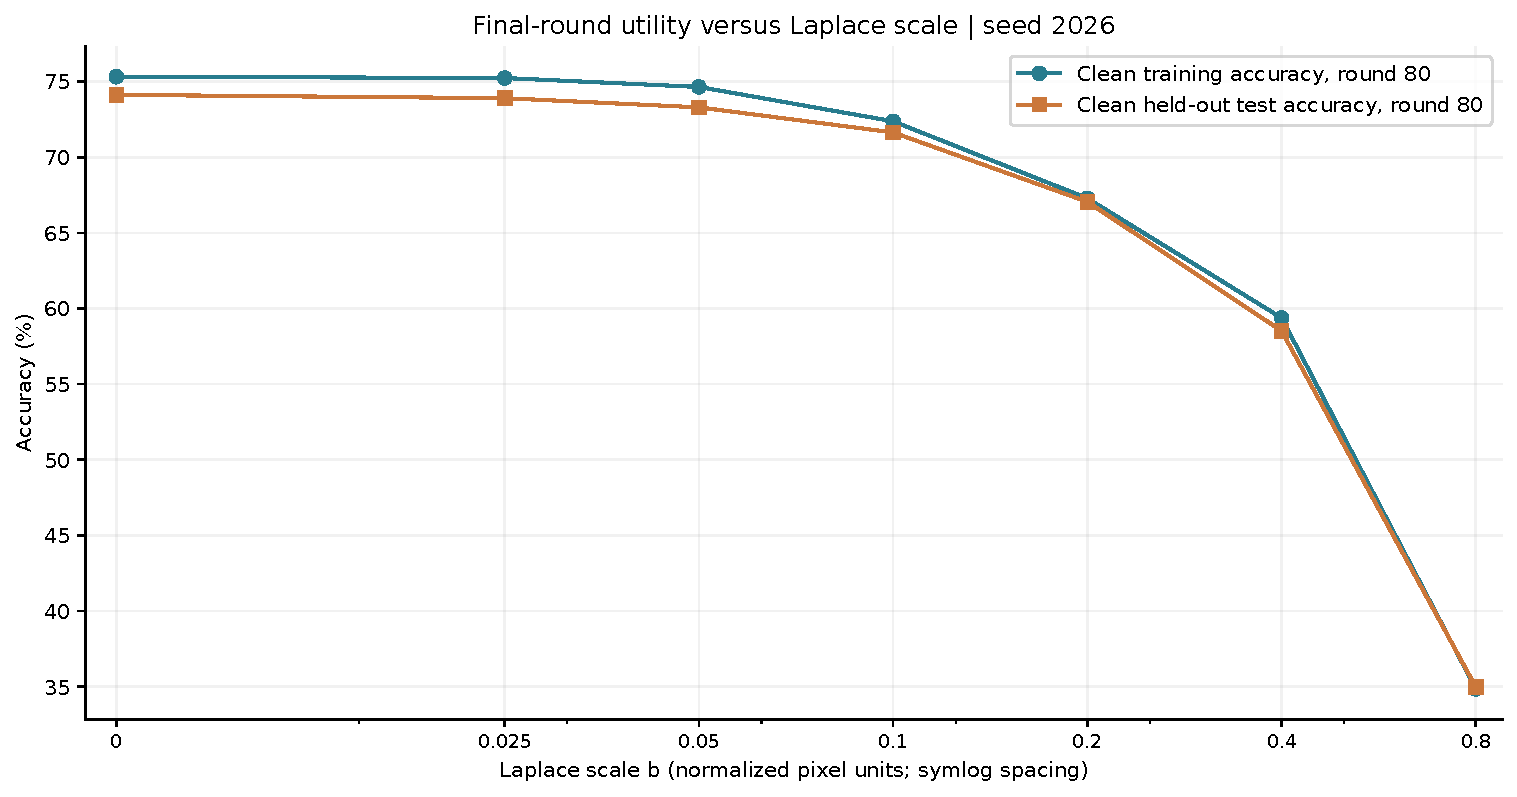
\includegraphics[width=0.9\linewidth]{figures/part2/dp_accuracy_vs_noise_scale.pdf}
\caption{Final clean training and test accuracy versus noise scale, seed 2026, round 80. The symlog axis is linear below $b=0.025$. Three-seed means appear in \cref{tab:noisegrid,fig:dpseeds}.}\label{fig:dpscale}
\end{figure}
\begin{figure}[htbp]
\centering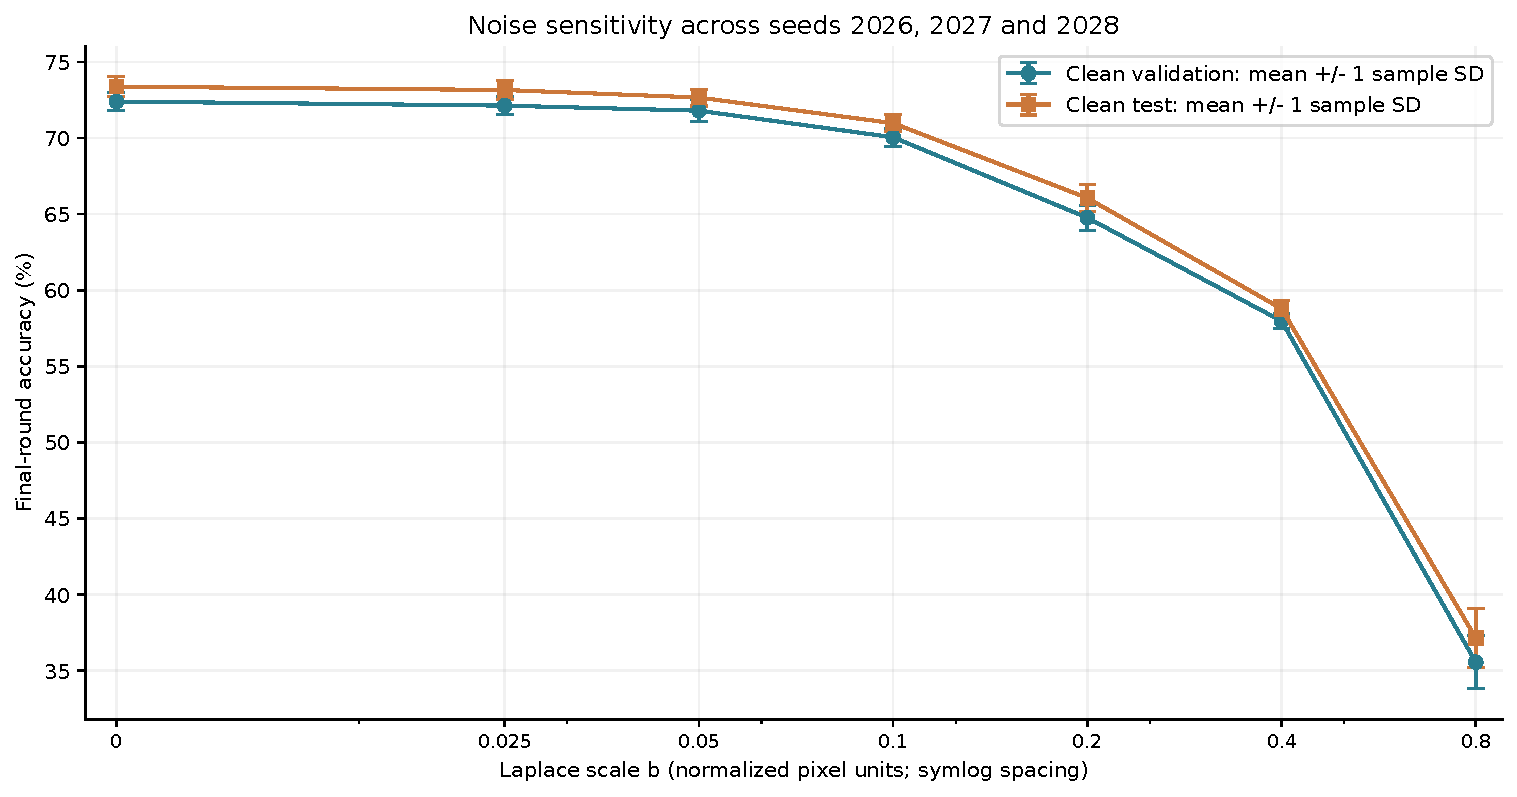
\includegraphics[width=0.9\linewidth]{figures/part2/dp_noise_seed_stability.pdf}
\caption{Mean final validation and test accuracy over three seeds, with sample-SD error bars. Every point uses round 80; no best-checkpoint results enter this plot. Larger error bars at $b=0.8$ indicate increased variation among these three training runs.}\label{fig:dpseeds}
\end{figure}

Training, validation, and test means decrease across the tested grid. Relative to the matched $b=0$ mean test accuracy of 73.38\%, $b=0.05$ loses 0.72 points and $b=0.8$ loses 36.22 points. The decline in both training and test accuracy indicates impaired signal learning under the fixed optimizer, rather than merely a wider generalization gap.

We adopted a two-percentage-point validation-accuracy tolerance as a practical utility constraint: it limits the absolute reduction in classification performance while allowing the strongest tested perturbation within that limit. This application-level choice is neither a statistical significance boundary nor a formal privacy requirement. We select the largest tested noise scale for which the mean final validation accuracy decreases by no more than two percentage points relative to the clean baseline:
\begin{equation}
\overline{A}_{\mathrm{val}}(0)-\overline{A}_{\mathrm{val}}(b)\le0.02,
\qquad A_{\mathrm{val}}\in[0,1].\label{eq:selection}
\end{equation}
The accuracy threshold is $72.39998\%-2\pp=70.39998\%$. At $b=0.05$, validation accuracy is 71.79647\%, a 0.60351-point decrease; at $b=0.10$, it is 70.04838\%, a 2.35159-point decrease. Thus \textbf{$b=0.05$ is the largest tested positive scale satisfying the criterion}, with pixel RMS distortion 0.07072 and mean test accuracy 72.65949\%. Test results describe this frozen choice and do not determine it.

Increasing $b$ from 0.10 to 0.20 reduces mean validation accuracy by a further 5.29 percentage points, from 70.05\% to 64.76\%, while mean test accuracy falls from 70.97\% to 66.06\%. Although larger $b$ tightens the hypothetical Laplace privacy bound for a fixed sensitivity, even these scales give very loose whole-image bounds (\cref{sec:privacy}). We therefore choose $b=0.05$ for the assignment's empirical distortion--utility comparison, not as a deployment recommendation for verified image-level privacy.

\subsection{Scientific Validation and Edge Cases}\label{sec:p2validation}
\subsubsection{Noise-law correctness: moments, quantiles, and tails}
Noise-law validation checks scale, shape, and tails against complementary Laplace properties:
\begin{equation}
\mathbb{E}[\xi]=0,\quad \mathbb{E}|\xi|=b,\quad
\operatorname{Var}(\xi)=2b^2,\quad
\Pr(|\xi|>3b)=e^{-3}.\label{eq:moments}
\end{equation}
At each of $b=0.025,0.10,0.80$, one million float32 draws are summarized in float64. Moments, seven quantiles between probabilities 0.01 and 0.99, and the $3b$ tail are checked against conservative six-standard-error thresholds. The mean SE is $\sqrt{2}b/\sqrt{N}$, the tail SE is $\sqrt{p(1-p)/N}$ for $p=e^{-3}$, and the variance SE is approximately $\sqrt{20}b^2/\sqrt{N}$, using fourth moment $24b^4$.

\begin{table}[htbp]
\centering
\caption{Million-sample distribution checks at each scale. The theoretical tail probability is $e^{-3}=0.0497871$ for all rows.}\label{tab:moments}
\begin{tabular}{rrrrr}
\toprule
$b$ & Empirical mean & Empirical variance & $2b^2$ & Empirical $3b$ tail\\
\midrule
0.025 & $-0.00001287$ & 0.00124851 & 0.00125000 & 0.049710\\
0.10 & $0.00001731$ & 0.01997336 & 0.02000000 & 0.049737\\
0.80 & $-0.00024118$ & 1.28365398 & 1.28000000 & 0.049780\\
\bottomrule
\end{tabular}
\end{table}

At $b=0.10$, empirical 0.01/0.99 quantiles are $-0.390109$/$0.389632$, versus theoretical $\mp0.391202$. The largest standardized quantile discrepancy is 1.578 at this scale and 2.003 across scales. All checked moment, quantile, and tail deviations are at most about 2.003 SE, within the six-SE bounds. Together, \cref{tab:moments,fig:noiselaw} discriminate incorrect scale or distribution shape more effectively than a mean-only check.

\begin{figure}[htbp]
\centering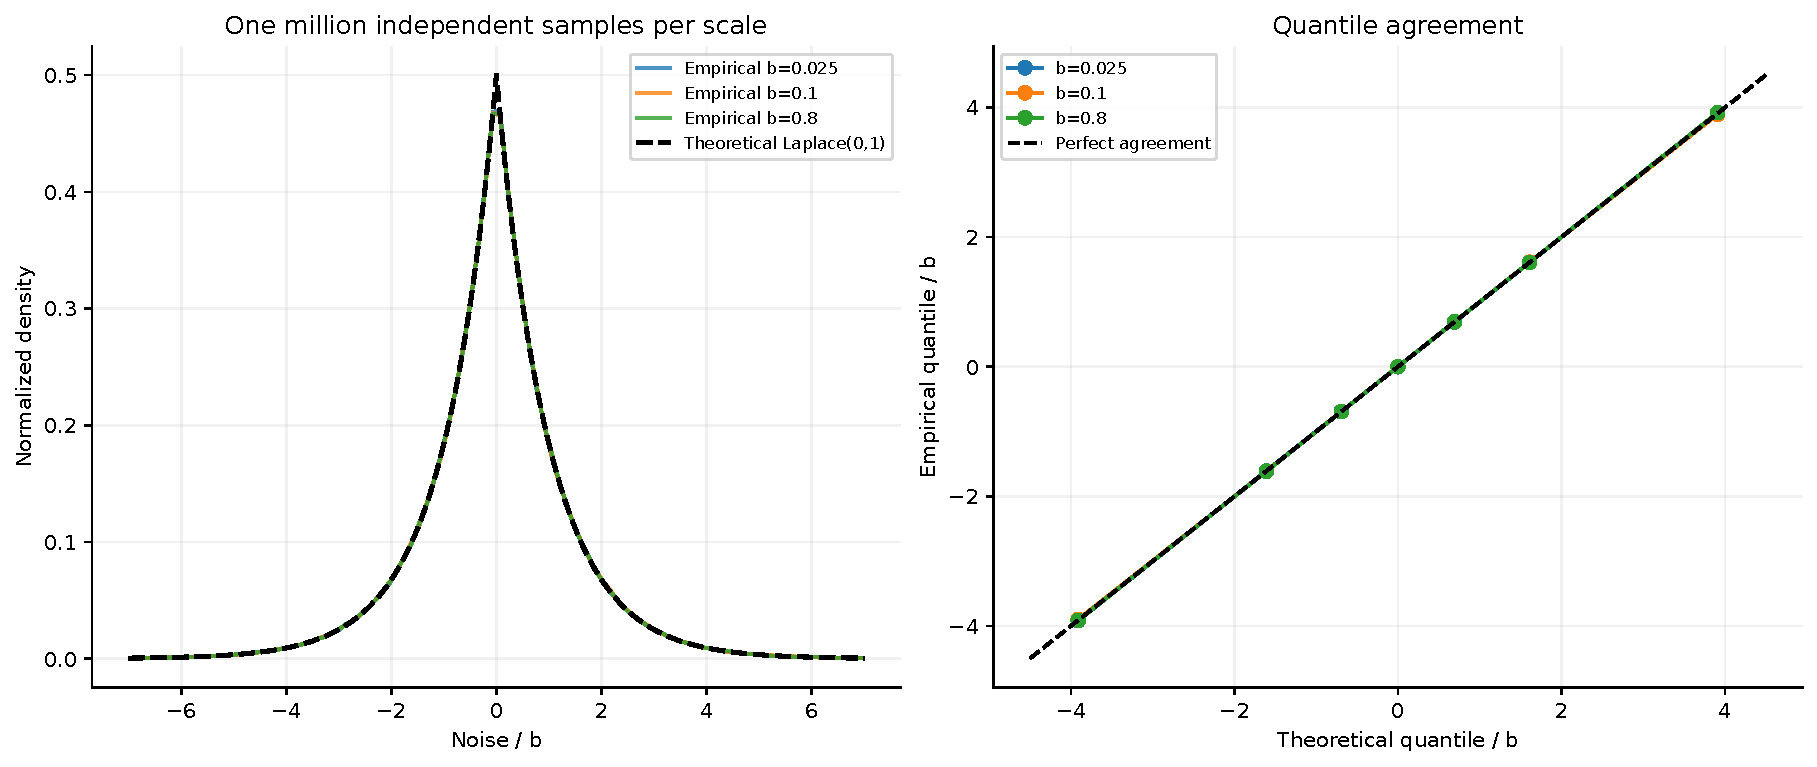
\includegraphics[width=\linewidth]{figures/part2/dp_noise_distribution_validation.pdf}
\caption{Mechanism validation: histograms of noise divided by $b$ against the unit-Laplace density, and empirical versus theoretical normalized quantiles. The three scales each use one million samples. Tail and moment checks in \cref{tab:moments} complement the plotted central density.}\label{fig:noiselaw}
\end{figure}

\subsubsection{Pixel independence, keyed reproducibility, and data isolation}
A broadcast scalar or shared-row noise bug would induce strong pixel correlations. Across 20,000 independent noise images, all 496 pairs among 32 spread pixel positions have maximum absolute correlation 0.020592, below $6/\sqrt{20{,}000}=0.042426$; mean correlation is $-0.000168$. This diagnostic detects no material linear dependence at the tested positions, while the sampling implementation supplies the IID construction.

Identical keys reproduce noise exactly; changed seeds or client IDs change it. CPU noise and its CUDA copy differ by 0.0, validating transfer rather than native-device PRNG equivalence. Two independent five-round runs at fixed $b=0.10$ also reproduce parameters and history metrics exactly.

Hash checks across all 100 clients confirm unchanged clean inputs, labels, validation tensors, and client boundaries. The held-out file hash is unchanged, computed without loading its examples during validation. Together with the separate frozen test phase, these checks verify that perturbation targets local training pixels only.

\subsubsection{Zero-noise equivalence as an end-to-end control}
The zero-noise control tests whether adding perturbation and evaluation code changes the clean algorithm. A three-round comparison matches initialization, schedules, optimizer settings, and batch seeds; parameter and all four metric differences are 0.0. The full $b=0$ runs then match their Part 1.1 counterparts for each seed 2026--2028: all 81 metric rows, 800 client selections, and round-80 parameters agree exactly.

This exact baseline recovery removes changes to splits or optimization as explanations for the positive-noise utility differences.

\subsubsection{Learning controls and noise-reuse ablation}
The synthetic noise control reaches a 100\% validation ceiling at every tested scale (\cref{app:synthetic_noise}), so the 21-run Federated EMNIST comparison provides the primary evidence for performance degradation.

To test sensitivity to noise reuse, matched 40-round real-data runs compare fixed perturbations with fresh noise each local epoch at $C=0.10,E=3$, learning rate 0.3, and batch size 32.
\begin{table}[htbp]
\centering
\caption{Separate fixed-versus-resampled-noise ablation. Values are final clean validation accuracy, using one matched seed and 40 rounds. No ablation result enters the main test grid.}\label{tab:ablation}
\begin{tabular}{rrrr}
\toprule
$b$ & Fixed (\%) & Fresh per local epoch (\%) & Difference (pp)\\
\midrule
0.10 & 64.8041 & 65.8342 & 1.0301\\
0.40 & 55.0804 & 60.1530 & 5.0726\\
\bottomrule
\end{tabular}
\end{table}
Fresh noise improves final validation accuracy by 1.03 points at $b=0.10$ and 5.07 at $b=0.40$ (\cref{tab:ablation}), suggesting that repeated exposure to fixed perturbations affects optimization. This single-seed ablation is separate from the primary fixed-noise test grid.

\subsubsection{Image distortion and client-level noise sensitivity}
Expected pixel MSE is $2b^2$, giving RMS $\sqrt{2}b$. At $b=0.05$, measured MSE/RMS are 0.00500156/0.0707217, close to 0.005/0.0707107; at $b=0.8$, RMS reaches 1.13127 (\cref{fig:distortion}). Out-of-range pixels rise from 47.10\% to 63.92\% across these scales. Even mild noise often crosses zero at background pixels, explaining the first fraction. \Cref{fig:images} illustrates the resulting image distortion.



\Cref{fig:robustness} shows each client's round-80 validation change from its same-seed $b=0$ control, averaged over three seeds and ordered by training-label entropy. Losses are widespread at larger scales but uneven: client 72 loses 8.93 points at $b=0.10$, while client 27 loses 68.33 at $b=0.8$.

\begin{figure}[htbp]
\centering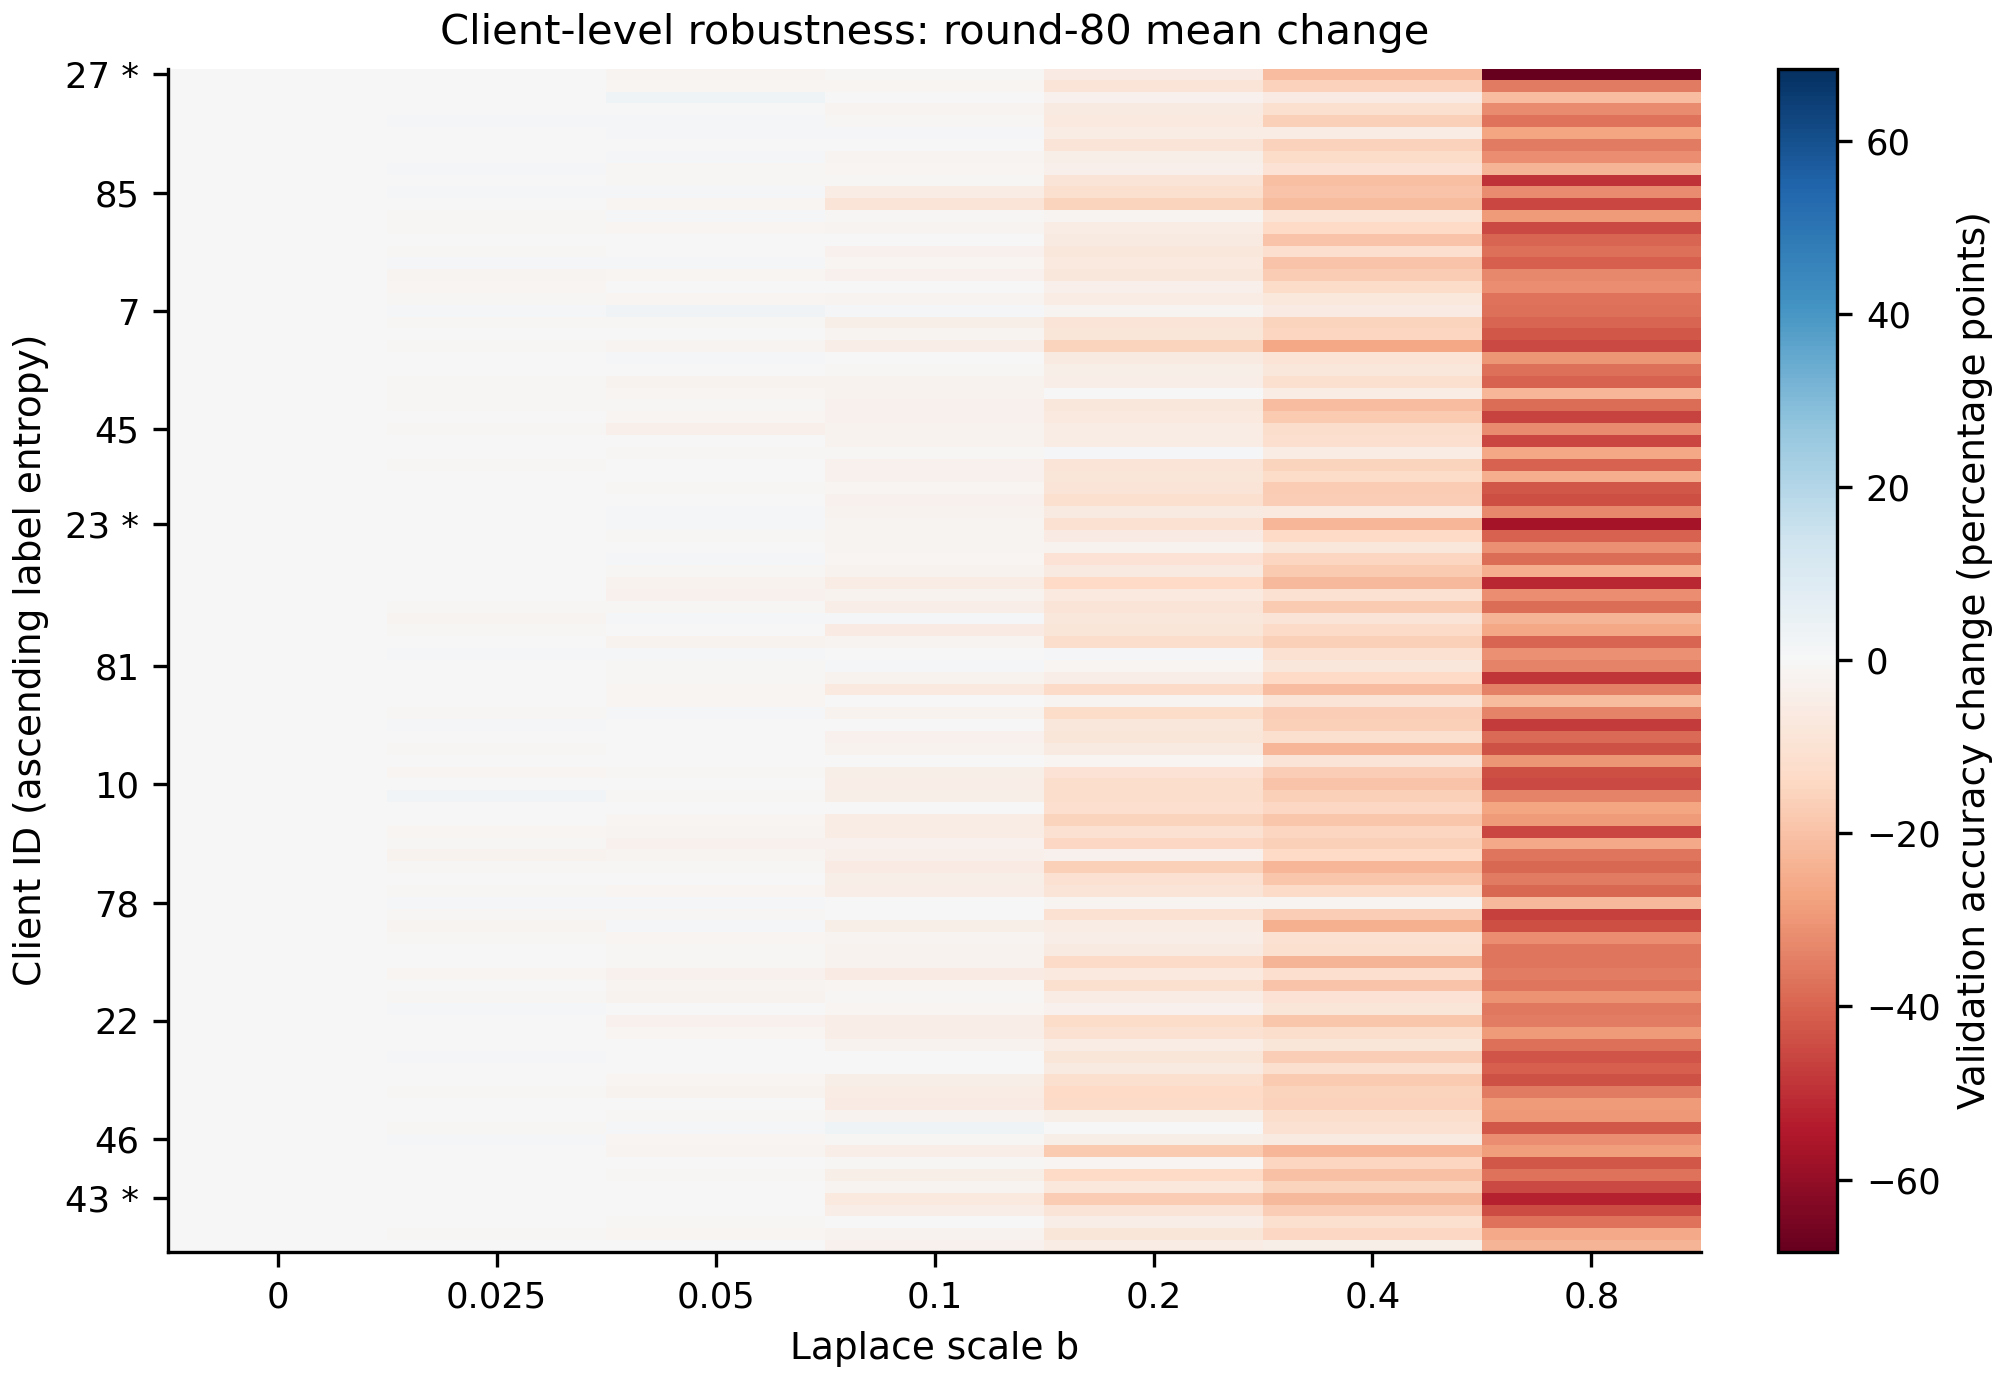
\includegraphics[width=\linewidth]{figures/part2/dp_client_robustness_heatmap.png}
\caption{Client-level changes in clean validation accuracy from matching $b=0$ controls, averaged over seeds 2026--2028 at round 80. Rows follow ascending training-label entropy. Stars mark clients 27, 23, and 43, the largest losses at $b=0.8$; the zero-noise column is identically zero.}\label{fig:robustness}
\end{figure}

Correlations of accuracy change with training size, entropy, and observed-class count are $-0.0385$, $-0.2305$, and $-0.2792$ at $b=0.10$, versus $-0.1743$, $0.0925$, and $-0.1477$ at $b=0.8$. Bottom/top size quartiles lose 34.60/39.22 points at $b=0.8$. The weak and changing associations describe heterogeneous sensitivity, without identifying a single causal predictor.

\subsubsection{Extreme noise, invalid inputs, and recovery}
Numerical stress tests distinguish finite deterioration from explicit failure. Client 25 trains for three local epochs at scales from $10^{-12}$ to $10^6$, with gradient and prediction monitoring and no clipping (\cref{tab:stress}). This is a local-update test, not a full federated trajectory.

\begin{table}[htbp]
\centering
\caption{Selected extreme-noise local stress outcomes on client 25. Finite confidence or loss does not imply valid classification.}\label{tab:stress}
\begin{tabularx}{\linewidth}{rYrr}
\toprule
$b$ & Outcome & Validation loss & Accuracy (\%)\\
\midrule
$10^{-12}$ & Finite; some float32 additions round away & 3.8003 & 4.17\\
1.6 & Finite & 3.9397 & 8.33\\
3.2 & Finite & 4.1622 & 0\\
10 & Finite; maximum $|\nabla|\approx1.07\times10^4$ & $1.19\times10^6$ & 0\\
100 & Finite; maximum $|\nabla|\approx1.12\times10^{13}$ & $9.03\times10^{22}$ & 0\\
1,000 & Explicit non-finite local-loss rejection & --- & ---\\
$10^6$ & Explicit non-finite local-loss rejection & --- & ---\\
\bottomrule
\end{tabularx}
\end{table}

At $b=10$, mean prediction confidence is 1.0 despite zero accuracy. At $b=1000$ and $10^6$, non-finite local loss is explicitly rejected and no failed update enters aggregation. Separate guards reject negative or non-finite scale, non-finite inputs, and float32 overflow.

A class-zero fixture with sizes $[0,1,2,7,101,23,3,9,11,13]$ tests empty/tiny clients, imbalance, missing classes, and interruption/resumption. Nine clients are eligible; resumed and uninterrupted parameters differ by 0.0. Client-specific keys regenerate the same fixed perturbations after restart.


\subsection{Privacy interpretation: what the experiment does and does not establish}\label{sec:privacy}
The course defines differential privacy through neighboring datasets and a bound on output-distribution changes \citep{courseDP}. For every neighboring pair $D\sim D'$ and measurable output set $A$, pure differential privacy requires
\begin{equation}
\Pr[M(D)\in A]\le e^{\varepsilon}\Pr[M(D')\in A].\label{eq:dp}
\end{equation}
For a query $f$ with specified sensitivity $\Delta_1f=\sup_{D\sim D'}\|f(D)-f(D')\|_1$, independent Laplace noise gives the classical calibration $\varepsilon=\Delta_1f/b$, or equivalently $b=\Delta_1f/\varepsilon$. Postprocessing preserves an already established guarantee, while multiple protected releases require an appropriate joint analysis or composition \citep{dworkroth2014}.

For an illustrative calibration, suppose the mechanism releases only one noisy normalized image, using independent, unpredictable private Laplace randomness, with no additional data-dependent outputs. Under \emph{pixel-level adjacency}, neighboring images differ in only one pixel by at most 1, so the identity query has $\Delta_1=1$ and $\varepsilon_{\mathrm{pixel}}=1/b$. At $b=0.05,0.10,0.20$, these values are 20, 10, and 5. Under \emph{whole-image replacement adjacency}, any image in $[0,1]^{784}$ may be replaced by another. The bound $\Delta_1\le784$ gives the worst-case calibration $\varepsilon_{\mathrm{image}}=784/b$: 15,680, 7,840, and 3,920 at the same scales, and 980 even at $b=0.80$. Thus the tested grid yields very loose worst-case whole-image guarantees for this hypothetical release; $b=0.05$ does not provide strong image-level privacy under this calibration.

These illustrative values are not privacy guarantees for the implemented FedAvg system. The experiment perturbs inputs rather than clipped gradients or model updates, and it implements no DP-SGD accountant. An end-to-end guarantee would require a protected unit (image or writer), adjacency relation, sensitivity bound, adversary model, and analysis of every released output.

Several outputs require protection beyond noisy images: labels, counts, and client IDs are unchanged; public reproducibility keys make noise reconstructible; and clean-data metrics access unperturbed examples. Multiple models, seeds, and metrics also enlarge the release surface. Fixed-noise reuse could invoke postprocessing only after establishing privacy for all information available to the learner and accounting for other releases. It does not automatically constitute a fresh release each epoch. Resampled noise requires a separate analysis.

Accordingly, $b=0.05$ remains the largest tested perturbation satisfying the predefined utility constraint. Its role is an empirical distortion--utility choice; deployment requiring verified image-level differential privacy would need a calibrated mechanism and complete accounting. No $\varepsilon$ is attributed to the actual trained FedAvg models or to the overall experimental pipeline.



\FloatBarrier
\section{Limitations and Scope of Interpretation}\label{sec:discussion}
The headline results use different protocols. Part 1.1 selects a seed and checkpoint with ten clients per round, whereas Part 1.2 uses four clients and selects round 78. Their 74.12\% and 73.79\% test accuracies therefore do not isolate a Ray effect; the matched four-client CPU comparison has zero metric difference. Part 2 reports three-seed round-80 means. Its appropriate clean comparator is 73.38\%, giving a 0.72-point mean test-accuracy decrease at $b=0.05$.

\Cref{tab:headlines} summarizes the headline results and their evaluation protocols, while \cref{tab:validation_summary} highlights the principal scientific validation evidence across the three parts.

\begin{table}[!htbp]
\centering
\caption{Headline outcomes with their evaluation protocols. The rows are descriptive summaries, not a controlled ranking of methods.}\label{tab:headlines}
\begin{tabularx}{\linewidth}{lYrY}
\toprule
Part & Method & Test accuracy & Protocol\\
\midrule
1.1 & Sequential FedAvg; ten clients/round & 74.12\% & Validation-selected seed 2026, round 80\\
1.2 & Ray CPU FedAvg; four clients/round & 73.79\% & Seed 2026, validation-selected round 78\\
2 & Sequential FedAvg + Laplace $b=0.05$ & 72.66\% & Mean round-80 accuracy over three seeds\\
\bottomrule
\end{tabularx}
\end{table}


\FloatBarrier
\paragraph{Statistical scope.}
The MLP, fixed learning rate, and 80-round budget define the tested regime. Three seeds characterize optimization variation on one split, not uncertainty across new writer populations; sample SDs are not confidence intervals. Selecting both settings and seeds on validation introduces selection optimism. Local validation estimates are coarse: one example changes client 25's accuracy by $100/24=4.17$ points. Class imbalance can obscure rare-label errors, and the aggregate test file does not establish writer-disjointness. Further tuning requires a new untouched test source.

\paragraph{Interpretation of controls.}
Partition reallocation holds sizes and exposures fixed but changes both label composition and assigned images, so the effect is not attributable to entropy alone. Client-benefit correlations are observational. Sampling frequencies and pixel correlations are finite diagnostics, not proofs of uniformity or independence; their thresholds use approximate sampling variation. The synthetic noise task is ceiling-limited, while extreme-noise tests cover one local workload. These limitations motivate the more discriminating controls in \cref{sec:plan}.

\begin{samepage}
\paragraph{Systems and privacy scope.}
Exact replay applies to the matched software/device environment. GPU equivalence covers one round; timings use three repeats on a shared host, and longer-term memory behavior is untested. Injected failures verify defined recovery paths rather than physical outages or arbitrary checkpoint-write failures. Shared-machine client separation does not establish network or filesystem security. The full privacy limitation is developed in \cref{sec:privacy}; utility and distortion measurements alone do not supply a formal DP guarantee.
\par
\end{samepage}

\begin{table}[!htbp]
\centering
\caption{Scientific validation across the three parts. The detailed experiments distinguish algebraic checks, controlled learning interventions, execution measurements, and stochastic diagnostics.}\label{tab:validation_summary}
\begin{tabularx}{\linewidth}{lYYY}
\toprule
Part & Validation question & Experiment & Main quantitative evidence\\
\midrule
1.1 & Are aggregation and local optimization correct? & Unequal-count average; one full-batch step versus centralized SGD & Errors $2.38\times10^{-7}$ and $7.45\times10^{-9}$\\
1.1 & Does learning respond to task structure? & Matched label randomization and partition interventions & Correct/shuffled: 66.36/7.65\%; homogeneous/segregated: 69.88/27.81\%\\
1.2 & Does Ray preserve the algorithm and run concurrently? & Matched 80-round trajectories; process intervals and cleanup & Parameter/metric differences 0.0; four overlapping Actors in 80/80 rounds\\
1.2 & Is parallel execution efficient? & Full matched workload, including startup and I/O & 11.95 s serial; 276.14 s Ray; speedup $0.0433\times$\\
2 & Does noise follow the specified law? & One million draws per scale; pixel-correlation checks & Variance 0.019973 versus 0.020000 at $b=0.1$; max $|r|=0.0206$\\
2 & Does perturbation preserve the clean baseline? & Full zero-noise replay at three seeds & All metrics, selections, and final parameters agree exactly\\
\bottomrule
\end{tabularx}
\end{table}
\FloatBarrier

\section{Three-Month Extended Validation Plan}\label{sec:plan}
The following proposed work targets the statistical, systems, and privacy gaps. Protocols would be fixed before evaluation, with a new untouched test source reserved for final confirmation.

\subsection{Month 1: statistical and algorithmic validation}
The first question is whether the observed configuration ordering and mild-noise utility loss persist beyond three seeds. Repeat paired comparisons over 10--20 seeds, then vary client splits separately. Report paired accuracy differences and uncertainty intervals, using client-cluster resampling for client-level outcomes. This separates optimization variability from data variability.

To distinguish improved optimization from additional computation, compare $(C,E)$ settings at both fixed communication rounds and fixed sample exposures or SGD steps. Cross learning rate with local epochs and a prespecified decay schedule. Measure time and communication proxy to a validation target, final accuracy, and local-update disagreement.

Replace the ceiling-limited signal task with varying signal amplitude, class separation, and informative-pixel counts. Independently manipulate client-size imbalance, label skew, and feature shift. Learning curves, rare-class recall, and excess error would reveal where perturbation or heterogeneity begins to impair learning.

\subsection{Month 2: parallel scalability and systems experiments}
Determine when local computation amortizes Actor overhead by varying model size, examples per client, participation, and local epochs under fixed resource budgets. Use at least ten independent Ray sessions per workload, timing startup, serialization, computation, synchronization, evaluation, and cleanup separately. Report speedup, time to target accuracy, CPU-seconds, peak memory, and the workload at which speedup exceeds one.

Compare ephemeral and persistent Actors under matched numerical controls; persistent Actors would be an extension, not a replacement for the assignment-required lifecycle. On isolated multi-node jobs, measure actual transferred bytes and latency under controlled bandwidth and delay. Test worker termination, driver restart, bounded memory pressure, and network disconnection. Recovery time, parameter agreement, duplicate/missing updates, and surviving processes would assess correctness beyond injected exceptions.

\subsection{Month 3: formal privacy analysis and robustness}
Define image- and writer-level adjacency, contribution bounds, the adversary's observations, and every model/metric release. Derive sensitivity and privacy accounting for fixed and resampled perturbations, then compare alternative local mechanisms and calibrated gradient/update perturbation under explicit trust assumptions. Validate the accountant independently and report utility against formal privacy budgets.

Complement the analysis with prespecified membership-inference and reconstruction tests, measuring attack AUC or low-false-positive-rate advantage and reconstruction error alongside classification utility. Attack failure would not constitute a privacy proof. Finally, introduce highly non-IID and adversarial clients to measure worst-client accuracy, rare-class recall, and rejection rates, separating robustness to malicious updates from privacy protection.

\section{Code Availability and Reproducibility}\label{sec:reproduction}
The source code, experiment configurations, and reproduction instructions are available at \url{https://github.com/yuxuanliang1/MLDS490-Assignment3}.

Run commands from the repository root. Place the instructor-provided \texttt{train\_data.npy} and \texttt{test\_data.npy} in \path{Assignment3-data/}, and reuse \path{part1_1_deepdish5_outputs/splits.json} for matched experiments. Dependencies are PyTorch, NumPy, Matplotlib, psutil (7.2.2), and Ray (2.60.0); the tested versions and hardware are given in \cref{sec:methodology}. The GPU experiments require a compatible CUDA build.

\Cref{app:reproduction} gives the ordered setup, training, selection, and test commands for each part. The principal scientific validation entry points are:
\begin{lstlisting}[language=bash]
cd MLDS490-Assignment3
python -m part1_1.run_tests
python -m part1_1 validate --device cuda:0
python -m part1_2.workflow validate
python -m part1_2.extra_validation
python -m part2.workflow math --device cuda:0
python -m part2.workflow science --device cuda:0
\end{lstlisting}
Part 1.1 covers algebraic, sampling, learning, and partition controls; Ray covers equivalence, benchmarks, and failure recovery; Part 2 covers the noise law, baseline recovery, ablations, and stress tests. Part 2's full zero-noise validation requires the completed Part 1.1 runs. Ray's validation includes GPU benchmarking even though CPU Actors are selected.

Completed results are stored under \path{part1_1_deepdish5_outputs/}, \path{part1_2_outputs/}, and \path{part2_outputs/}. Figures can be regenerated without training:
\begin{lstlisting}[language=bash]
python -m part1_1 plots
python -m part1_2.workflow artifacts
python -m part2.workflow artifacts
python report/tools/regenerate_figures.py
\end{lstlisting}
The final command renders the report-sized plots from saved numerical outputs. The image-distortion panel also requires development images. Completed runs and frozen test evaluations are cached; use a separate output/project copy for a fresh repetition. The \texttt{run\_server.sh} and \texttt{finalize\_server.sh} launchers contain DeepDish5-specific configuration; consult the corresponding repository README before using them on another host.

\section{Conclusion}\label{sec:conclusion}
Sequential FedAvg achieves 74.12\% held-out accuracy, with aggregation and centralized-SGD checks agreeing to float32 precision. Label randomization and controlled heterogeneity produce large, interpretable changes in validation accuracy. Ray preserves the matched CPU trajectory and executes four clients concurrently in every round, but lifecycle overhead makes this workload approximately 23.1 times slower than sequential execution.

Fixed Laplace perturbation reduces clean utility as scale increases. The largest tested positive scale causing no more than a two-percentage-point decrease in mean final validation accuracy is $b=0.05$: validation accuracy decreases from 72.40\% to 71.80\%, and mean round-80 test accuracy is 72.66\%. Distribution, zero-noise, and recovery checks validate the implemented experiment; an end-to-end privacy guarantee still requires the formal analysis outlined above.

\FloatBarrier
\bibliographystyle{plainnat}
\bibliography{references}
\clearpage
\appendix
\section{Supplementary Comparisons}\label{app:supplement}
\subsection{Communication-round results versus local computation}
\Cref{fig:cost} compares the six settings by cumulative client-epochs. Unequal client sizes make sample exposures in \cref{tab:grid} a more precise computation measure.

One float32 model occupies $108{,}478\times4=433{,}912$ parameter bytes. An uncompressed download-plus-upload proxy is $2mT(433{,}912)$ bytes for $m$ participants and $T$ rounds, excluding protocol overhead and retries.
\begin{figure}[htbp]
\centering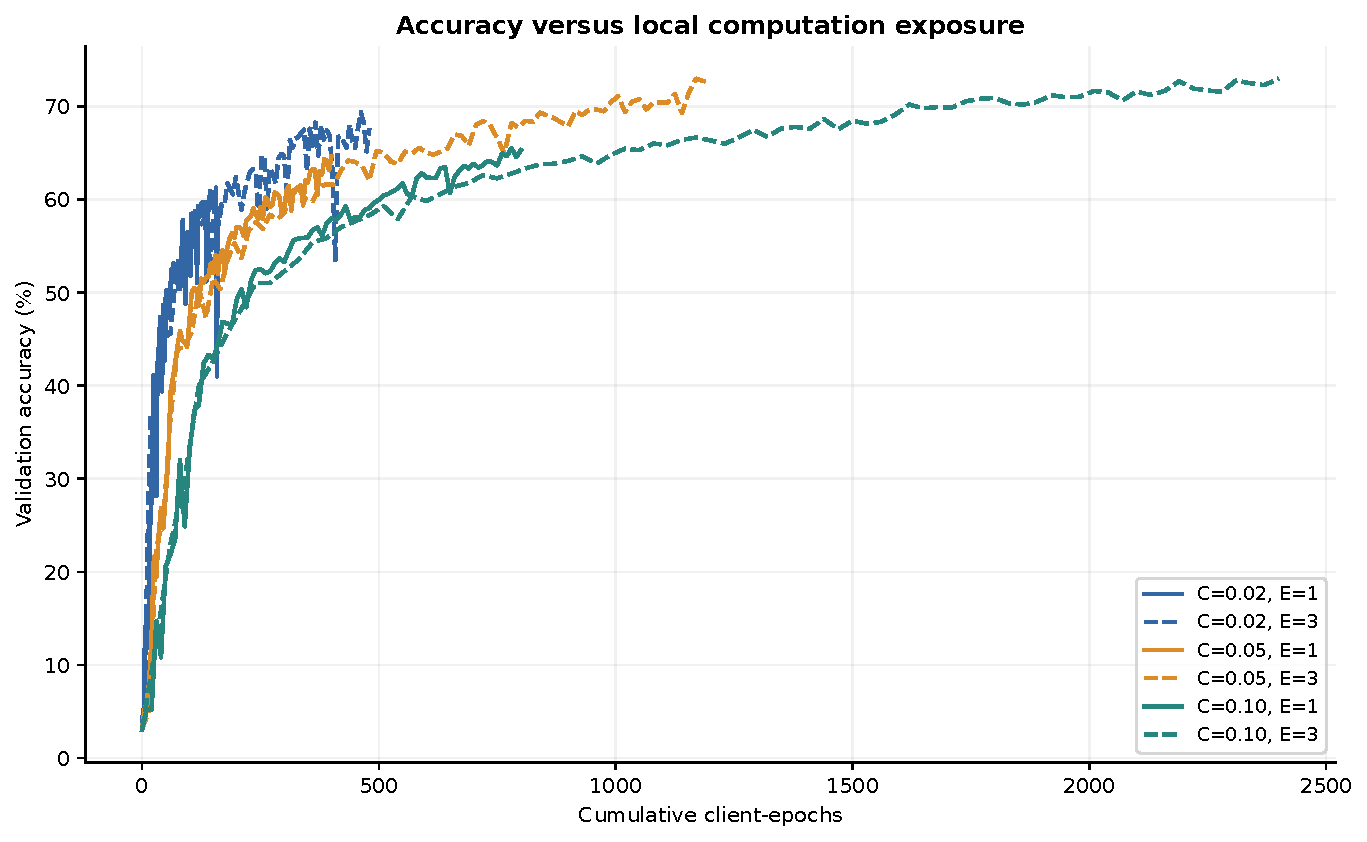
\includegraphics[width=0.9\linewidth]{figures/part1_1/accuracy_vs_client_epochs.pdf}
\caption{Validation accuracy versus cumulative client-epochs for the six seed-2026 configurations. Curves terminate at different budgets because all runs stop after 80 rounds.}\label{fig:cost}
\end{figure}

\subsection{Seed variability in the leading FedAvg settings}
\Cref{fig:seeds} shows pointwise mean validation accuracy and sample SD across three fixed-split seeds. Selection uses mean best validation across seeds, rather than the best point of this mean trajectory.
\begin{figure}[htbp]
\centering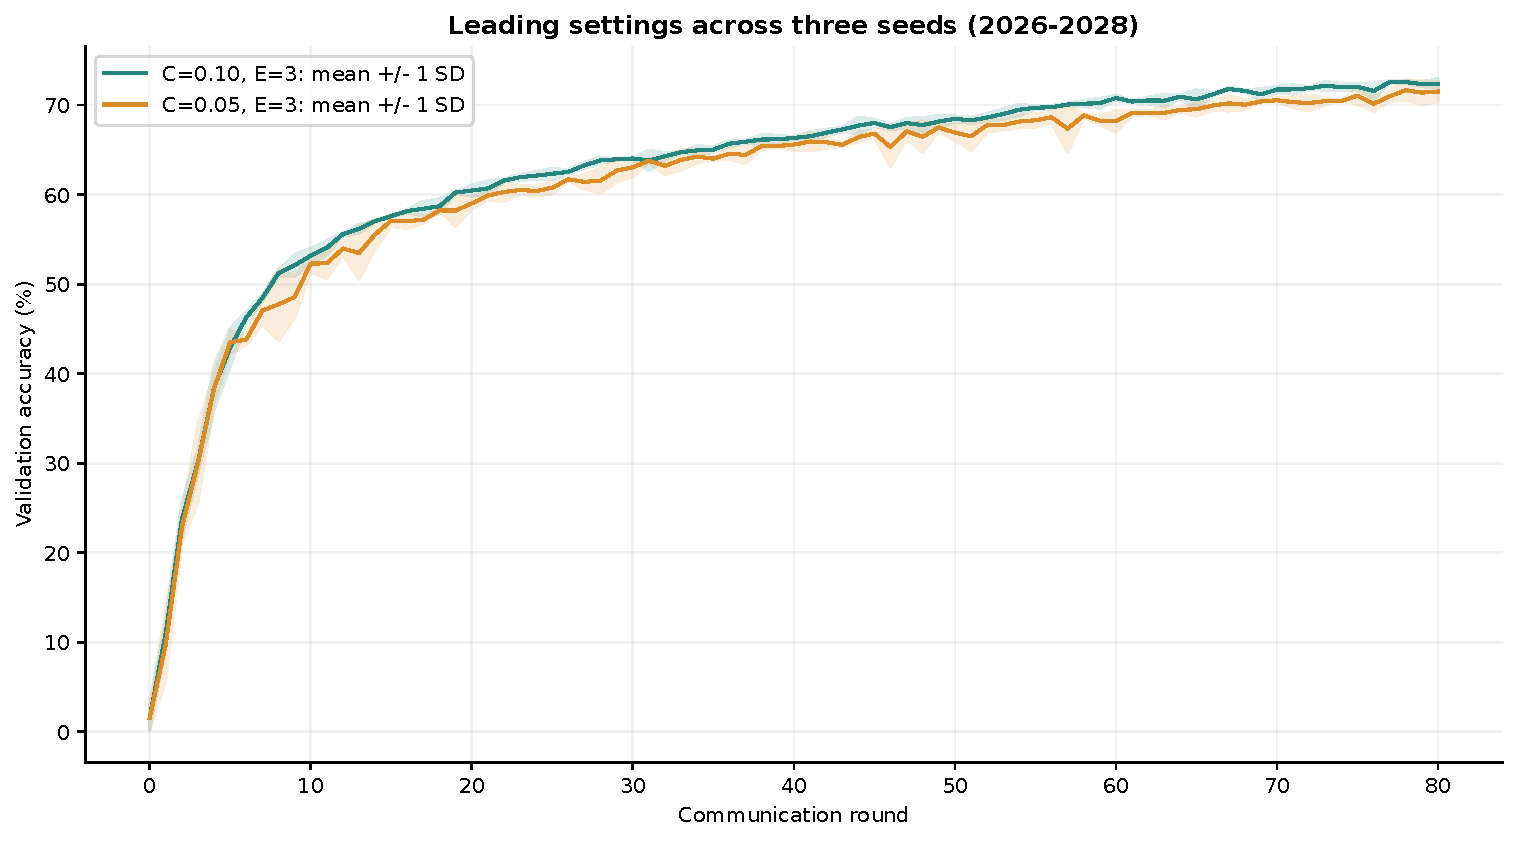
\includegraphics[width=0.9\linewidth]{figures/part1_1/seed_stability.pdf}
\caption{Leading sequential settings at $E=3$, seeds 2026--2028. Shading is one pointwise sample SD; the split remains fixed.}\label{fig:seeds}
\end{figure}

\subsection{Matched serial and Ray trajectories}
\Cref{fig:raymatch} displays the matched four-client CPU comparison: training and validation trajectories coincide, with maximum metric difference 0.0.
\begin{figure}[htbp]
\centering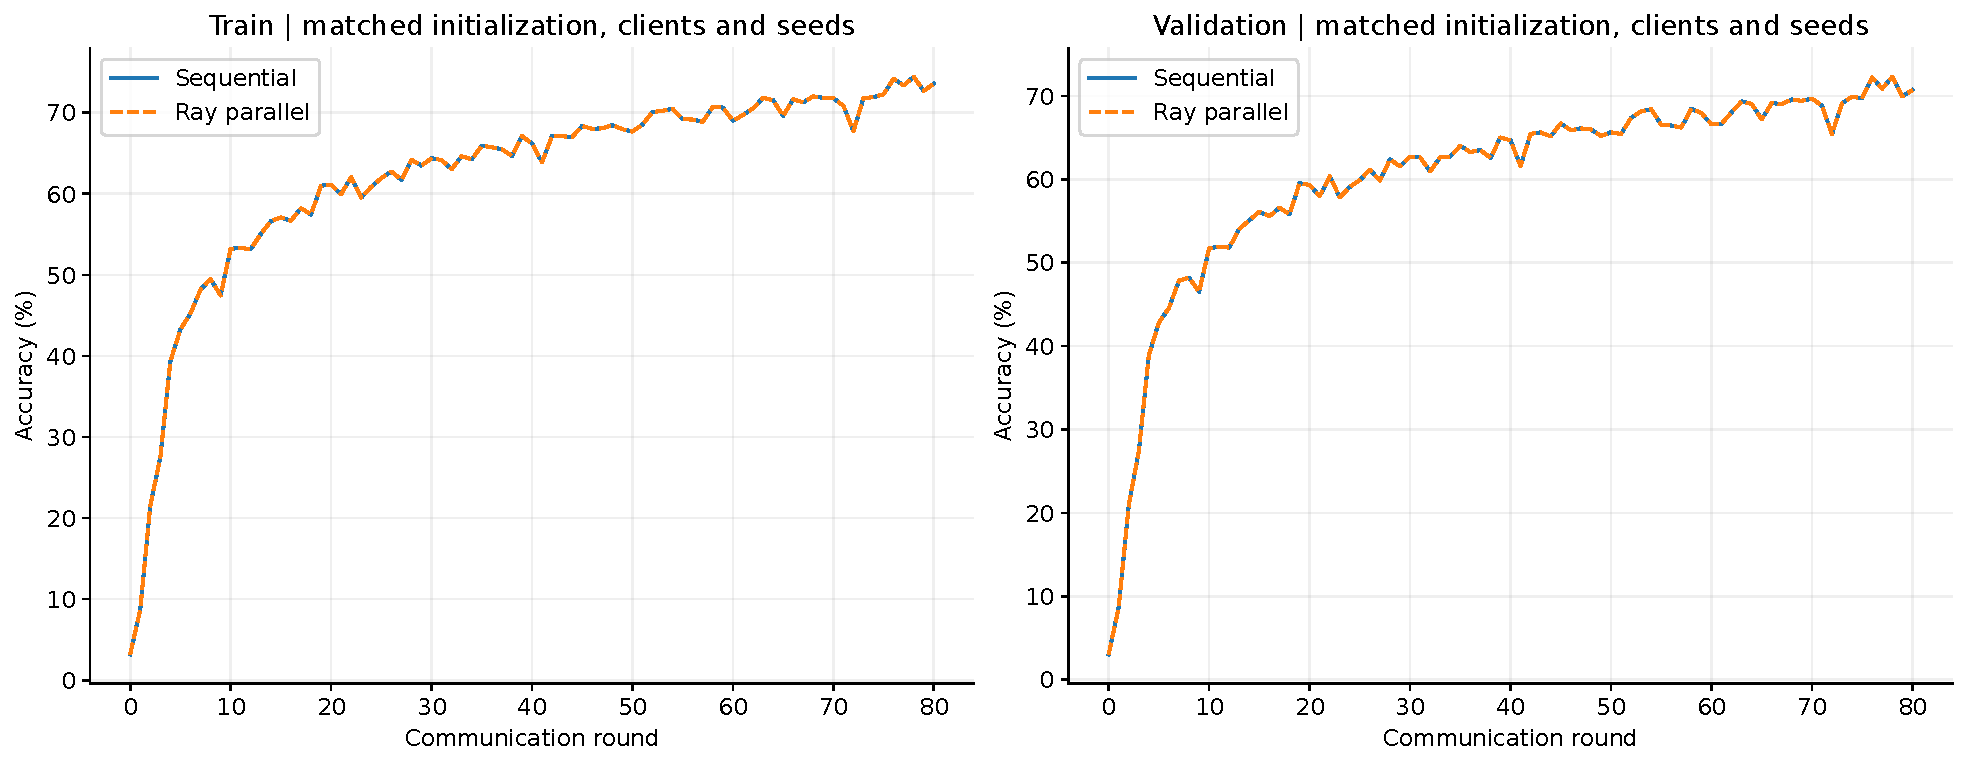
\includegraphics[width=\linewidth]{figures/part1_2/sequential_parallel_accuracy.pdf}
\caption{Matched 80-round sequential and Ray CPU accuracy trajectories, seed 2026, four clients per round. Initial parameters, selections, local minibatches, optimizer settings, and aggregation order are identical.}\label{fig:raymatch}
\end{figure}

\subsection{Distortion is a mechanism diagnostic, not a privacy budget}
\Cref{fig:distortion} relates measured RMS to $\sqrt{2}b$ and mean validation accuracy. Its horizontal axis is perturbation magnitude, not a privacy budget.
\begin{figure}[htbp]
\centering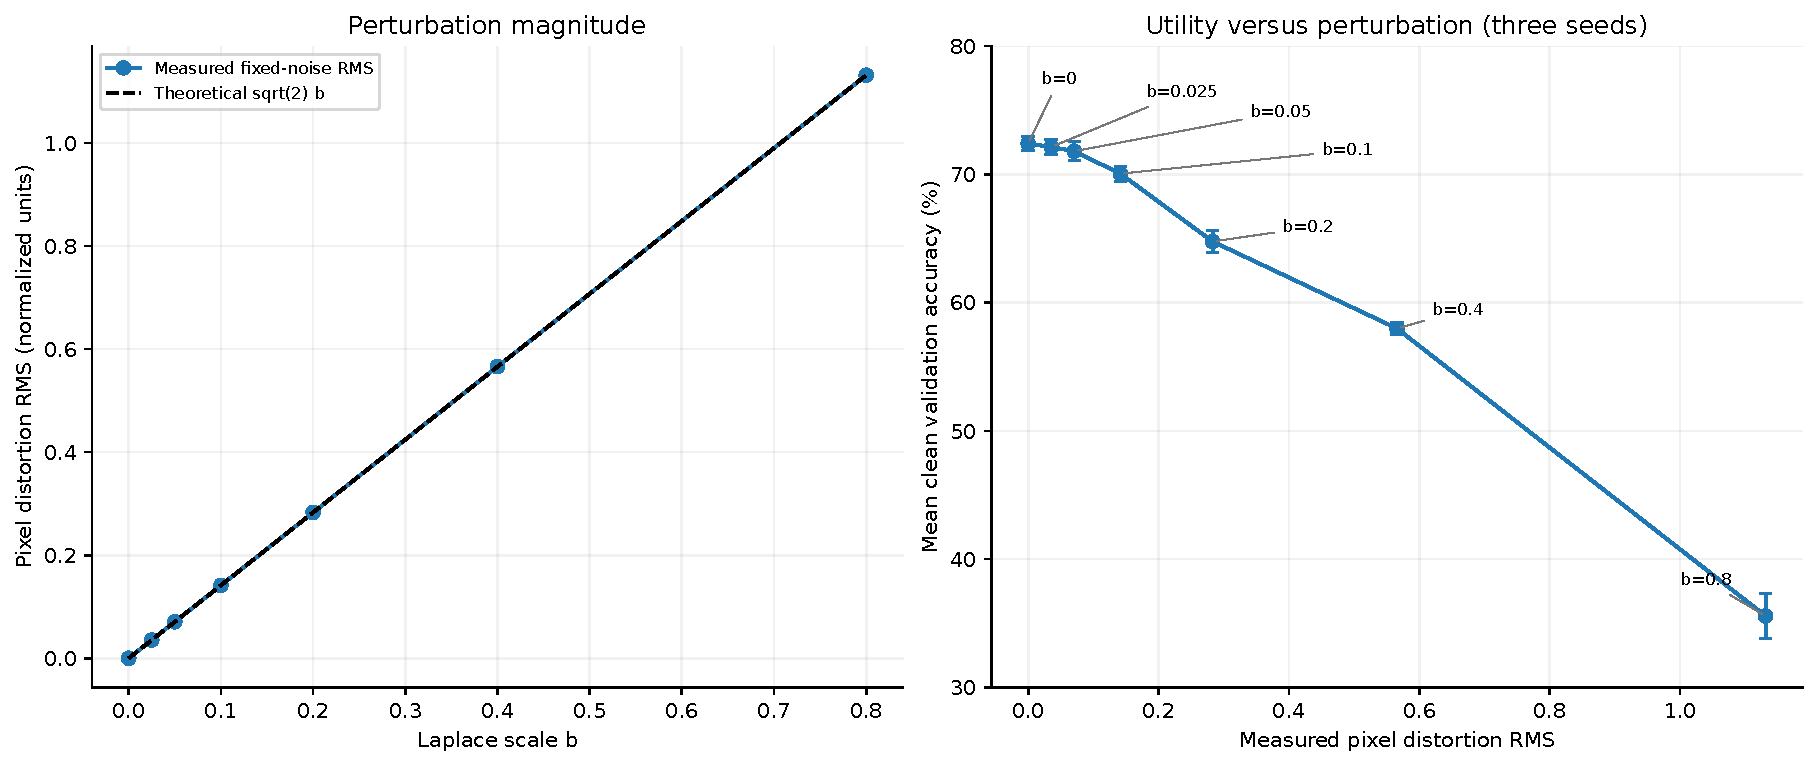
\includegraphics[width=\linewidth]{figures/part2/dp_privacy_utility_tradeoff.pdf}
\caption{Measured RMS distortion versus theory (left), and three-seed mean round-80 clean validation utility versus measured RMS (right). Error bars are sample SD. Annotations identify the tested scales.}\label{fig:distortion}
\end{figure}


\section{Supporting Perturbation Diagnostics}\label{app:noise_diagnostics}
The clean cross-entropy curves complement Question 1's accuracy comparison. The image panel shows how increasing noise alters the same four training images; saturation applies only to display.
\begin{figure}[htbp]
\centering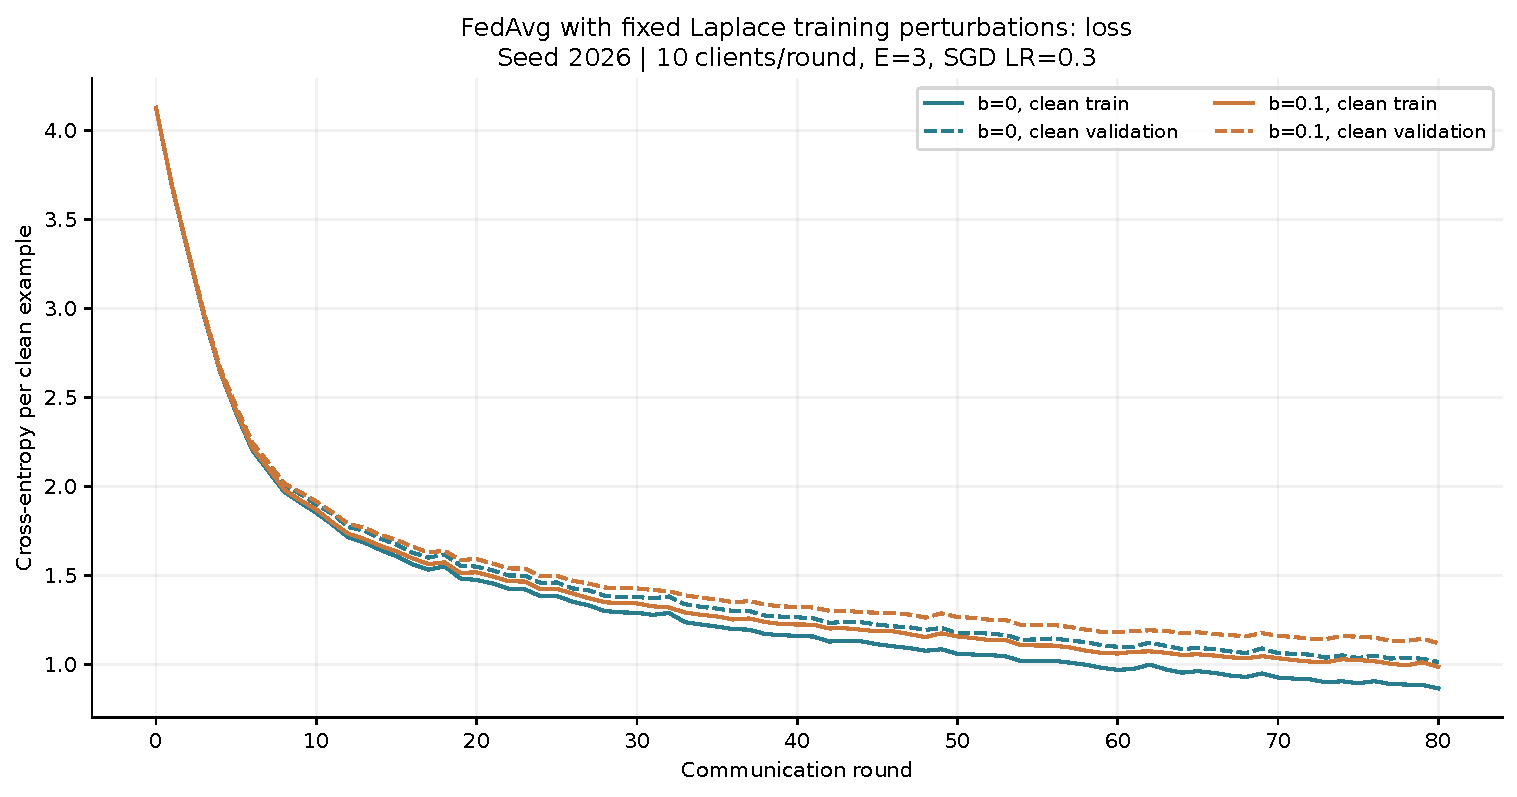
\includegraphics[width=0.9\linewidth]{figures/part2/dp_loss_convergence.pdf}
\caption{Clean-data cross-entropy for the same matched runs as \cref{fig:dpaccuracy}. The positive-noise run learns but retains higher clean training and validation loss. These are evaluation losses, not losses measured on the perturbed local batches.}\label{fig:dploss}
\end{figure}

\begin{figure}[htbp]
\centering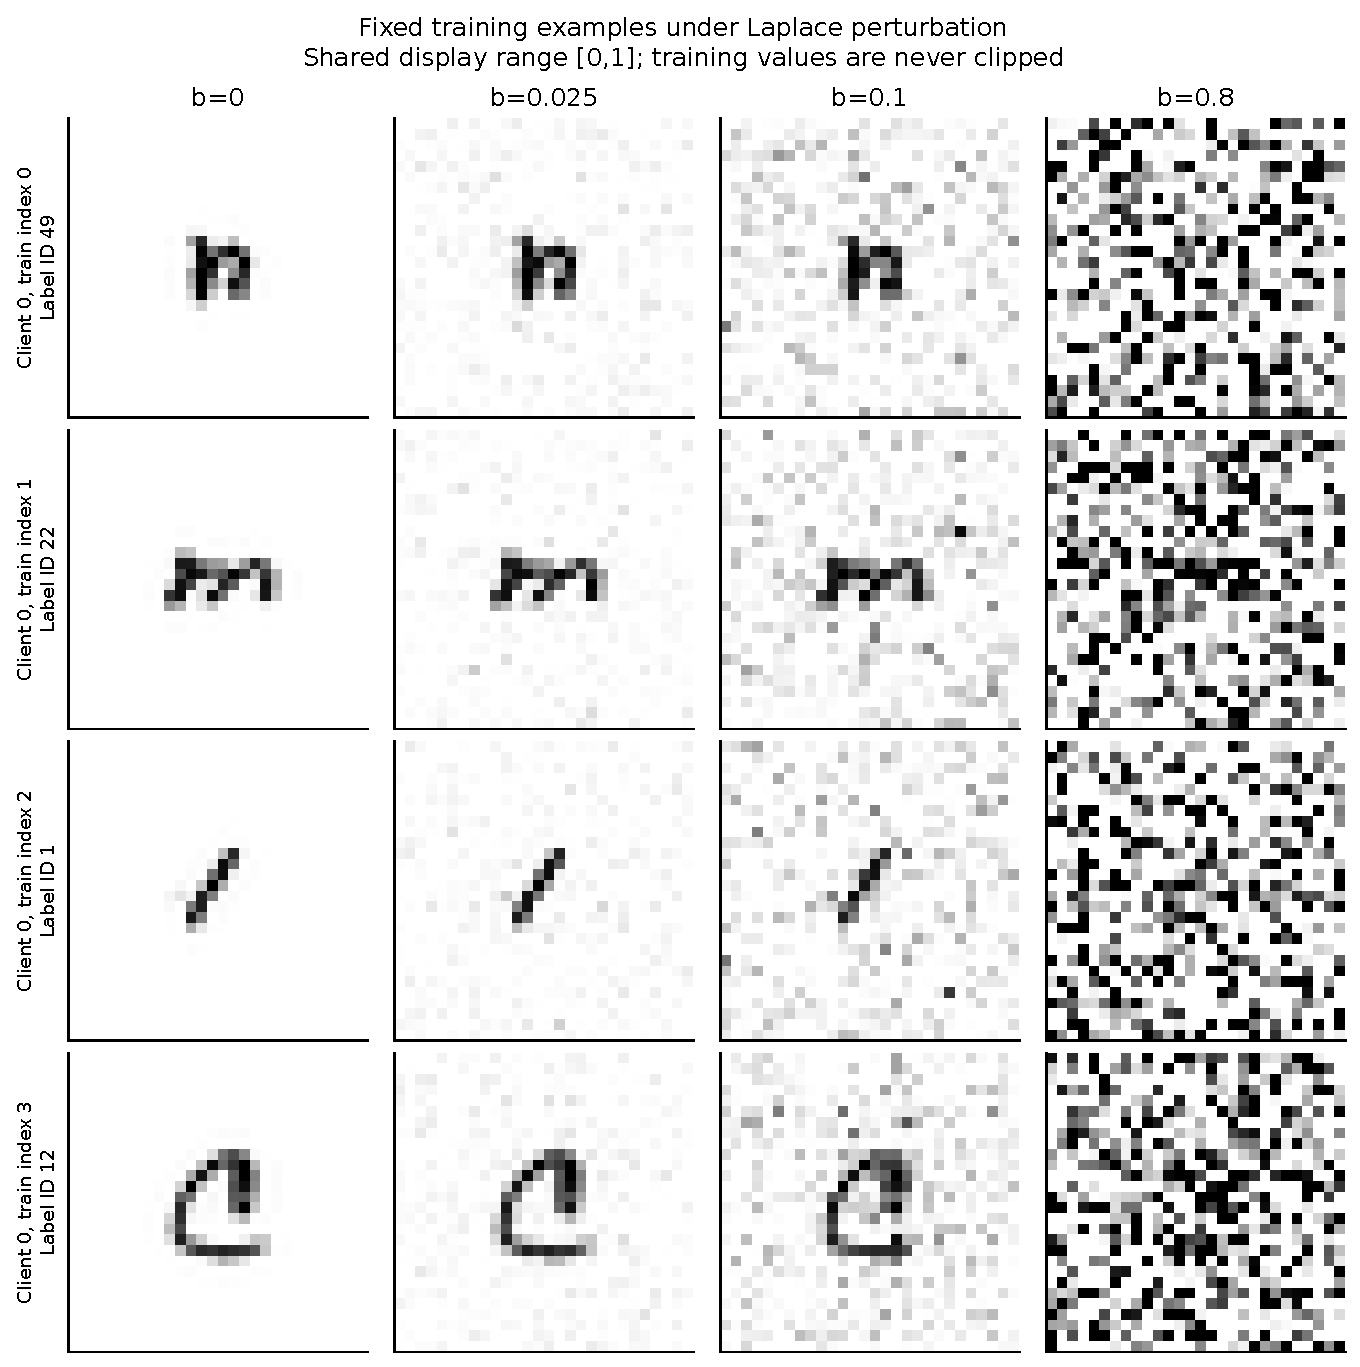
\includegraphics[width=0.76\linewidth]{figures/part2/dp_image_perturbations.pdf}
\caption{Four client-0 training examples at $b=0,0.025,0.10,0.80$, seed 2026. Display values saturate at $[0,1]$; training inputs are never clipped. Labels are numeric class IDs.}\label{fig:images}
\end{figure}

\FloatBarrier
\subsection{Ceiling-limited synthetic noise control}\label{app:synthetic_noise}
A controlled spatial-signal classification task tested whether increasing noise weakens learning. Twenty clients supplied 480 training and 160 validation examples. Seeds 371--373 were each run at $b=0,0.2,2.0$ for 30 rounds, with $E=1$ and learning rate 0.1. All nine runs achieved 100\% clean-validation accuracy across the three noise scales and three seeds. This ceiling effect prevents the task from distinguishing noise-induced degradation and cannot establish robustness to perturbation. The real Federated EMNIST grid in \cref{tab:noisegrid} provides the primary evidence for performance degradation.

\section{All Seed-Specific Final-Round Noise Results}\label{app:allnoise}
\begin{longtable}{rrrrrr}
\caption{All 21 round-80 outcomes. Accuracy is in percent; correct counts refer to the clean held-out test partition.}\label{tab:allnoise}\\
\toprule
$b$ & Seed & Clean train & Clean validation & Test & Correct / 3,621\\
\midrule
\endfirsthead
\toprule
$b$ & Seed & Clean train & Clean validation & Test & Correct / 3,621\\
\midrule
\endhead
\bottomrule\endfoot
0 & 2026 & 75.32 & 73.00 & 74.12 & 2,684\\
0 & 2027 & 74.83 & 72.33 & 72.88 & 2,639\\
0 & 2028 & 74.76 & 71.87 & 73.13 & 2,648\\
0.025 & 2026 & 75.23 & 72.81 & 73.90 & 2,676\\
0.025 & 2027 & 74.64 & 71.89 & 72.80 & 2,636\\
0.025 & 2028 & 74.62 & 71.69 & 72.77 & 2,635\\
0.05 & 2026 & 74.64 & 72.64 & 73.29 & 2,654\\
0.05 & 2027 & 73.80 & 71.39 & 72.27 & 2,617\\
0.05 & 2028 & 74.02 & 71.36 & 72.41 & 2,622\\
0.1 & 2026 & 72.37 & 70.72 & 71.64 & 2,594\\
0.1 & 2027 & 72.01 & 69.74 & 70.67 & 2,559\\
0.1 & 2028 & 72.10 & 69.69 & 70.62 & 2,557\\
0.2 & 2026 & 67.28 & 65.49 & 67.05 & 2,428\\
0.2 & 2027 & 66.54 & 64.94 & 65.84 & 2,384\\
0.2 & 2028 & 65.81 & 63.85 & 65.29 & 2,364\\
0.4 & 2026 & 59.38 & 58.37 & 58.52 & 2,119\\
0.4 & 2027 & 58.41 & 57.42 & 58.44 & 2,116\\
0.4 & 2028 & 58.95 & 58.14 & 59.40 & 2,151\\
0.8 & 2026 & 34.86 & 33.57 & 34.99 & 1,267\\
0.8 & 2027 & 37.65 & 36.88 & 38.66 & 1,400\\
0.8 & 2028 & 37.80 & 36.24 & 37.81 & 1,369\\
\end{longtable}

\Cref{tab:allnoise} gives the seed-specific outcomes underlying \cref{tab:noisegrid}. Each model is evaluated at round 80 on the same 3,621 test examples. Question 1 uses the seed-2026 $b=0.10$ validation-best checkpoint, which also occurs at round 80.

\section{Complete Reproduction Commands}\label{app:reproduction}
These Bash commands run from the repository root after dataset placement and installation of the versions in \cref{sec:methodology}. Select an available GPU through the host's normal allocation procedure. Parts 1.1 and 2 accept \texttt{--device cpu}; reproducing the GPU comparisons requires CUDA. The shared split manifest is reused throughout.

\begin{lstlisting}[language=bash]
export CUBLAS_WORKSPACE_CONFIG=:4096:8 MPLBACKEND=Agg
export OMP_NUM_THREADS=2 MKL_NUM_THREADS=2 OPENBLAS_NUM_THREADS=2
# Part 1.1: data analysis, pilot, grid, and scientific validation
python -m part1_1.run_tests
for phase in inspect pilot suite validate; do
  python -m part1_1 "$phase" --device cuda:0
done
python -m part1_1.audit
# Freeze selection before accessing test data
for phase in select test plots report; do
  python -m part1_1 "$phase" --device cuda:0
done
python -m part1_1.audit --final
\end{lstlisting}
The pilot selects the shared learning rate, the suite includes leading-setting seed repeats, and validation executes the controls in \cref{sec:p11validation}. For a separate configurable run, copy the split manifest into the new output directory first:
\begin{lstlisting}[language=bash]
python -m part1_1 train --device cpu --rounds 80 \
  --fraction 0.10 --epochs 3 --lr 0.3 --batch-size 32 \
  --seed 2026 --threads 2 --name controlled_run \
  --output-dir new_outputs
\end{lstlisting}

Ray requires one thread per process. Preparation creates client-specific training files; validation includes numerical comparisons and three-repeat CPU/GPU benchmarks. Training runs the matched trajectories and evaluates the validation-selected model:
\begin{lstlisting}[language=bash]
export OMP_NUM_THREADS=1 MKL_NUM_THREADS=1 OPENBLAS_NUM_THREADS=1
python -m part1_2.workflow prepare
python -m part1_2.workflow validate
python -m part1_2.extra_validation
python -m part1_2.workflow train
python -m part1_2.workflow artifacts
python -m part1_2.audit
\end{lstlisting}

Part 2 uses the completed Part 1.1 baselines for full zero-noise validation. The scientific phase includes synthetic controls, fixed/resampled-noise ablations, and recovery/stress tests. All 21 final checkpoints and the separate Question 1 checkpoint are evaluated only after the pretest audit and protocol freeze:
\begin{lstlisting}[language=bash]
export OMP_NUM_THREADS=2 MKL_NUM_THREADS=2 OPENBLAS_NUM_THREADS=2
for phase in init math pilot grid science; do
  python -m part2.workflow "$phase" --device cuda:0
done
python -m part2.audit --pretest
python -m part2.workflow freeze
python -m part2.workflow test --device cuda:0
python -m part2.workflow artifacts
python -m part2.workflow audit
\end{lstlisting}
Completed configurations and test results are cached. Fresh repetitions should use separate output/project copies. On interruption, each workflow restores the last committed checkpoint; Part 2 regenerates fixed perturbations from their client keys.

\end{document}
